

% \begin{figure*}[ht]
% % \vspace{-4mm}
% \centering     %%% not \center
% \subfigure[Homogeneous (uniform)]{\label{fig:a}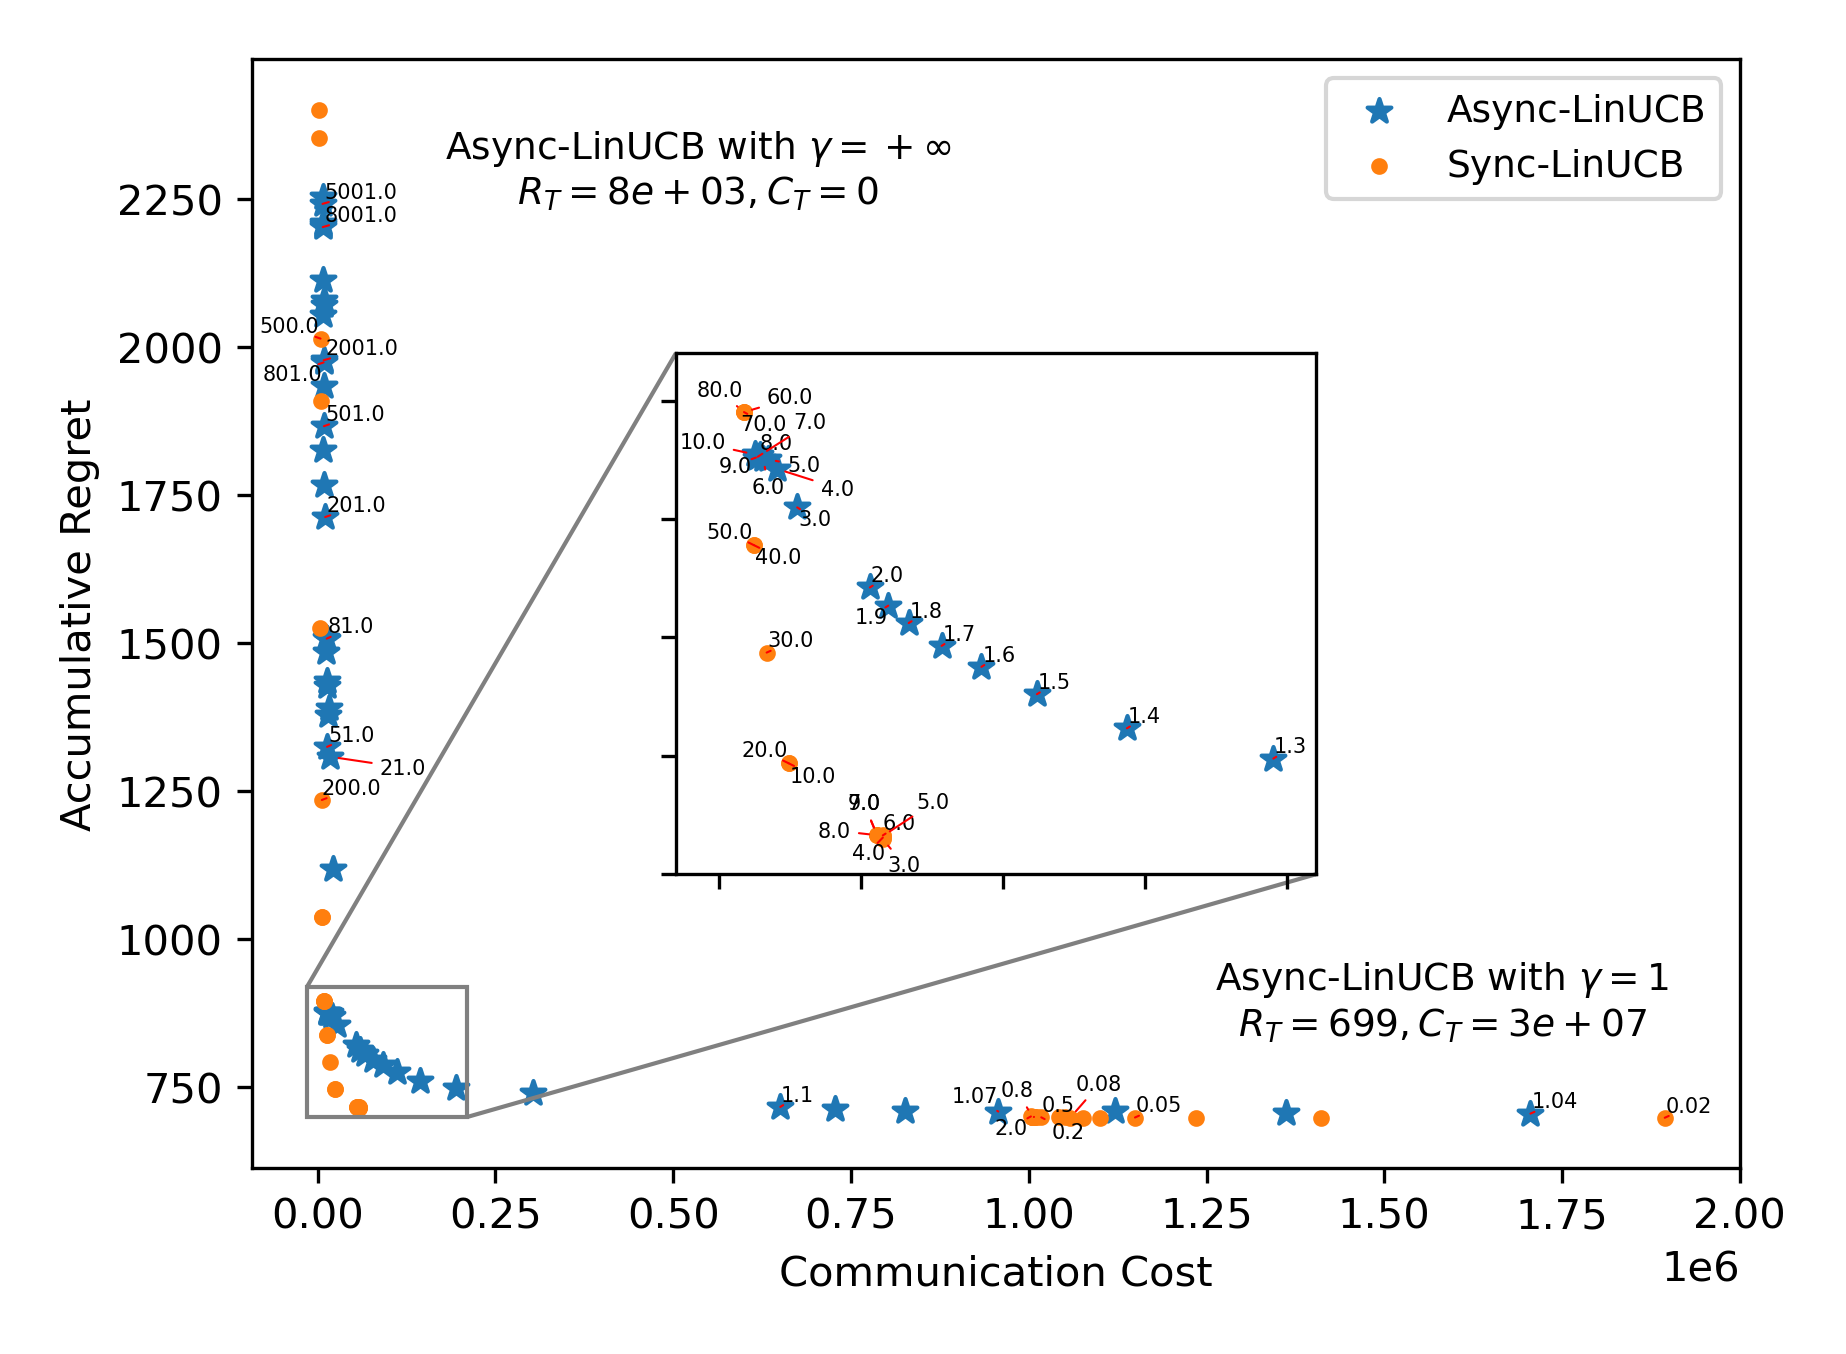
\includegraphics[width=0.32\textwidth]{imgs/regretVScommCost_uniform_noclutter.png}}
% \subfigure[Homogeneous (non-uniform)]{\label{fig:b}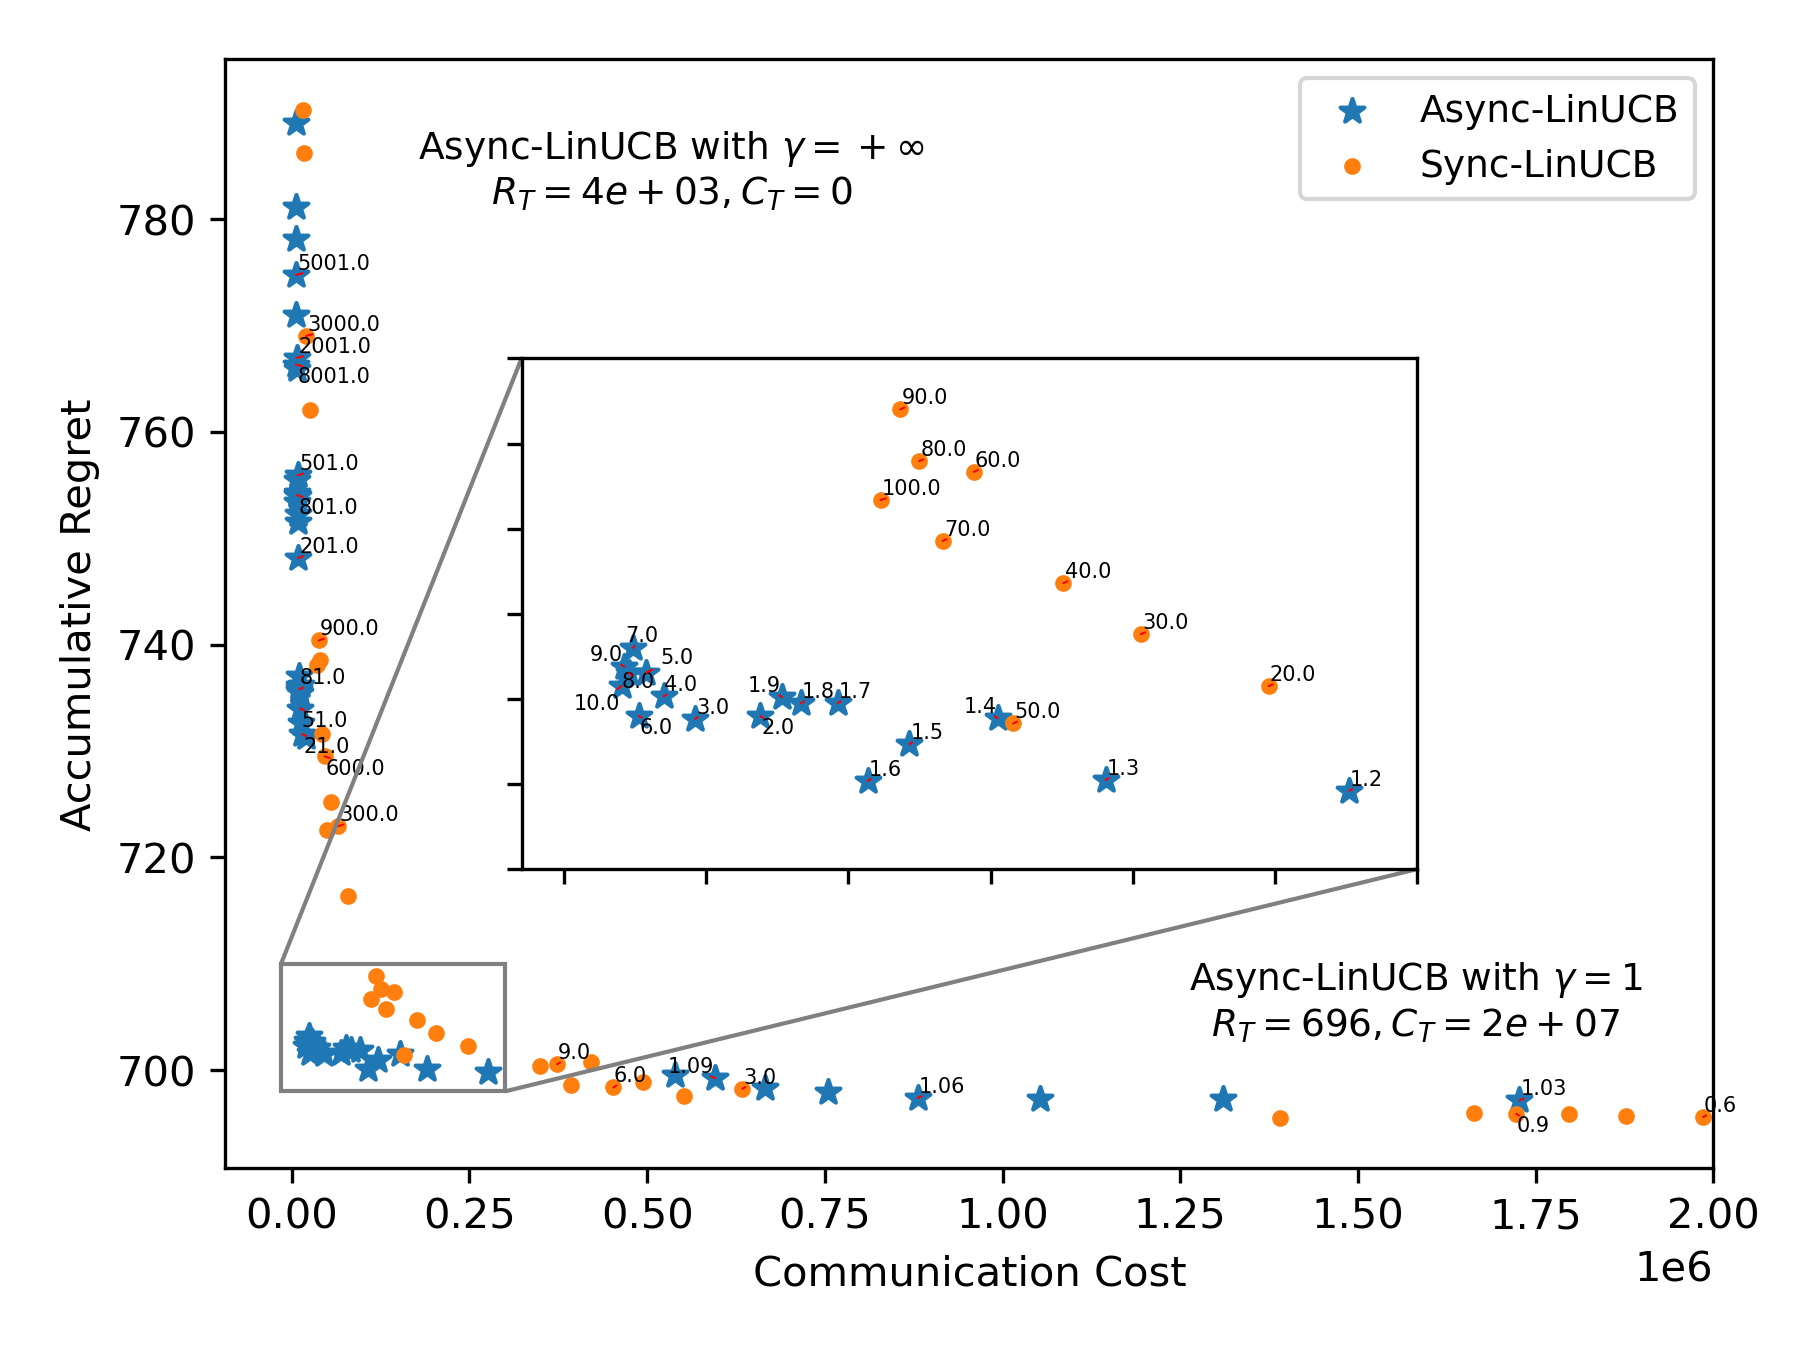
\includegraphics[width=0.32\textwidth]{imgs/regretVScommCost_nonuniform_noclutter.png}}
% \subfigure[Heterogeneous clients]{\label{fig:c}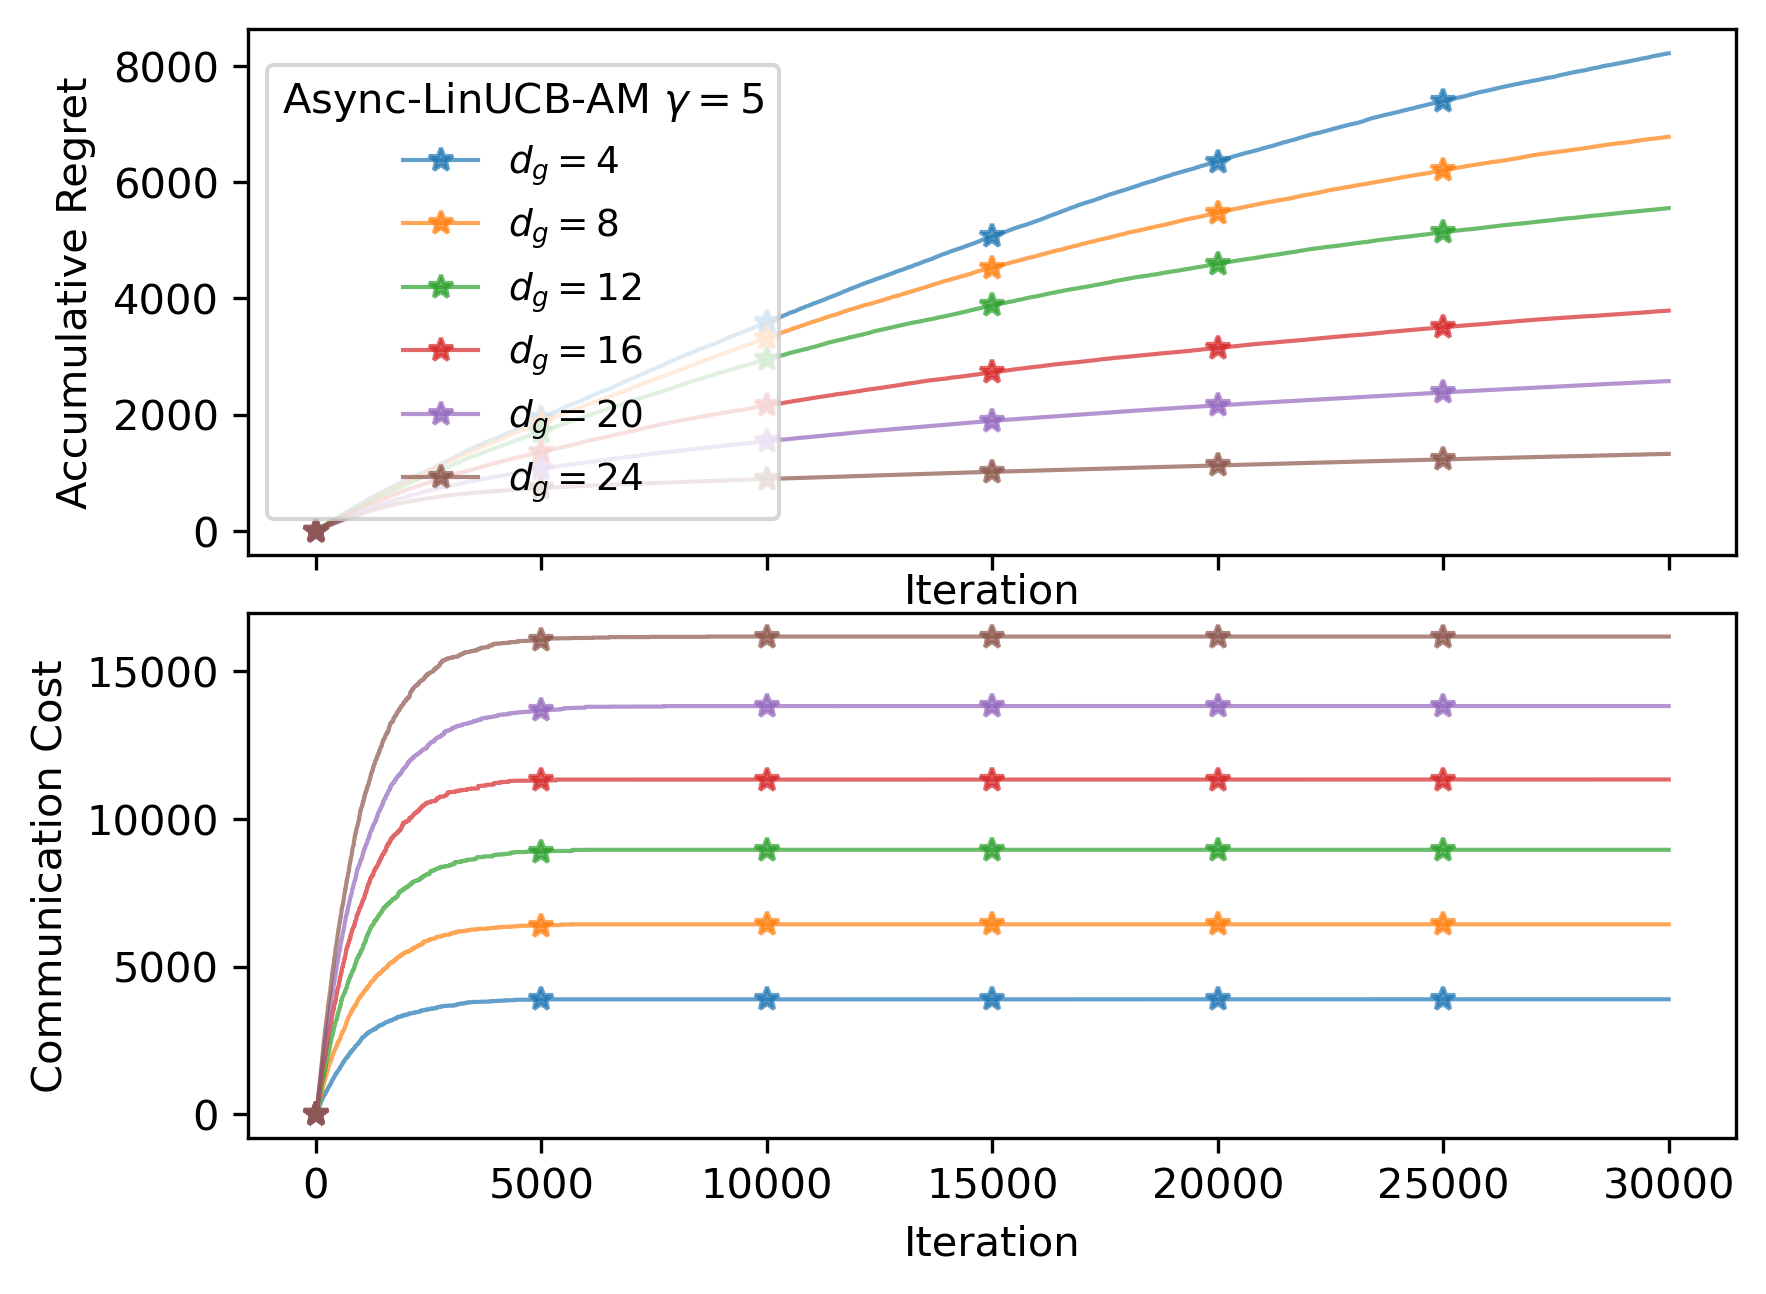
\includegraphics[width=0.31\textwidth]{imgs/sim_hetero_30000.png}}
% % \vspace{-3mm}
% \medskip
% % \vspace{-2.5mm}
% \subfigure[LastFM ($N=1892$)]{\label{fig:d}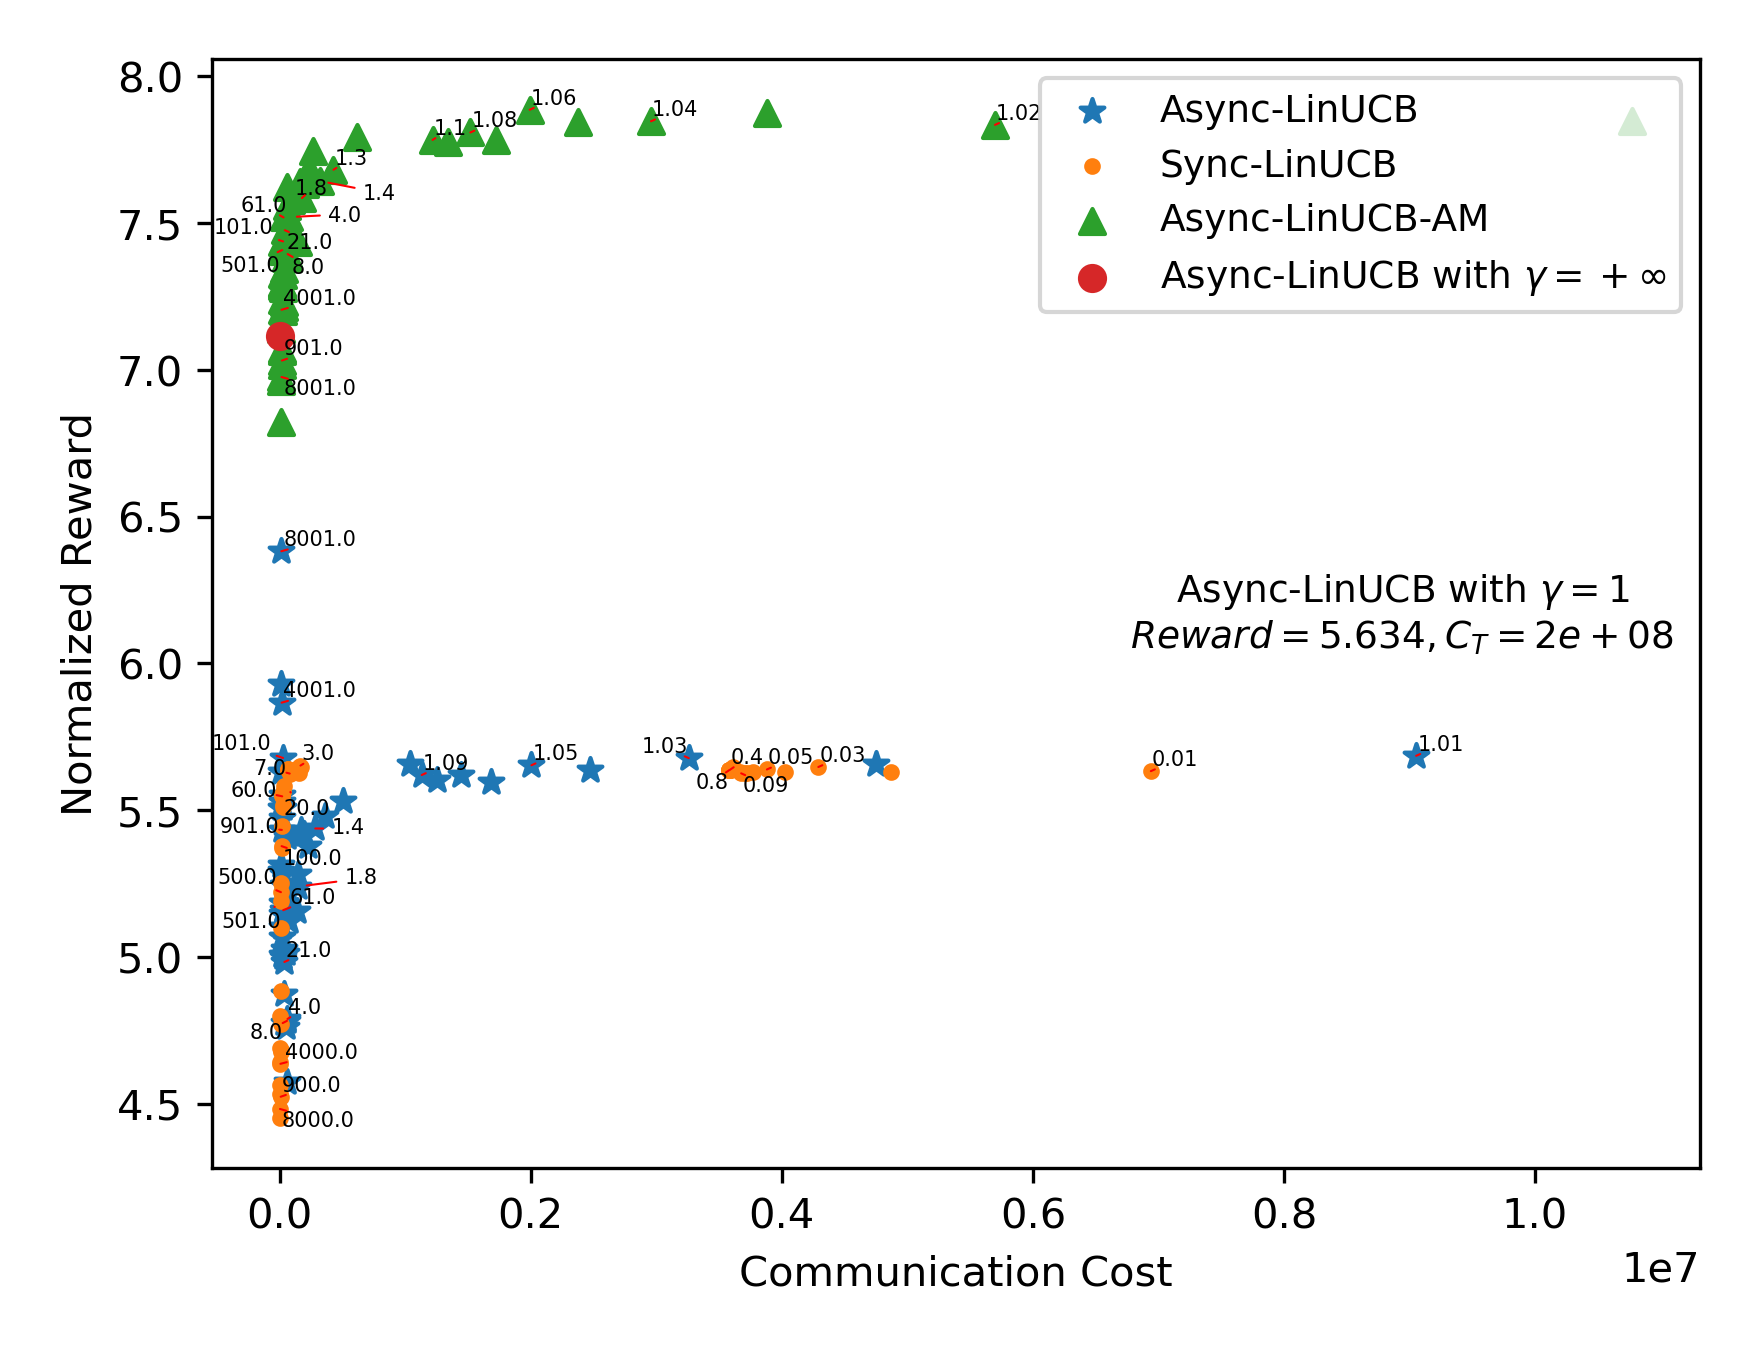
\includegraphics[width=0.32\textwidth]{imgs/regretVScommCost_lastfm_noclutter.png}}
% \subfigure[Delicious ($N=1867$)]{\label{fig:e}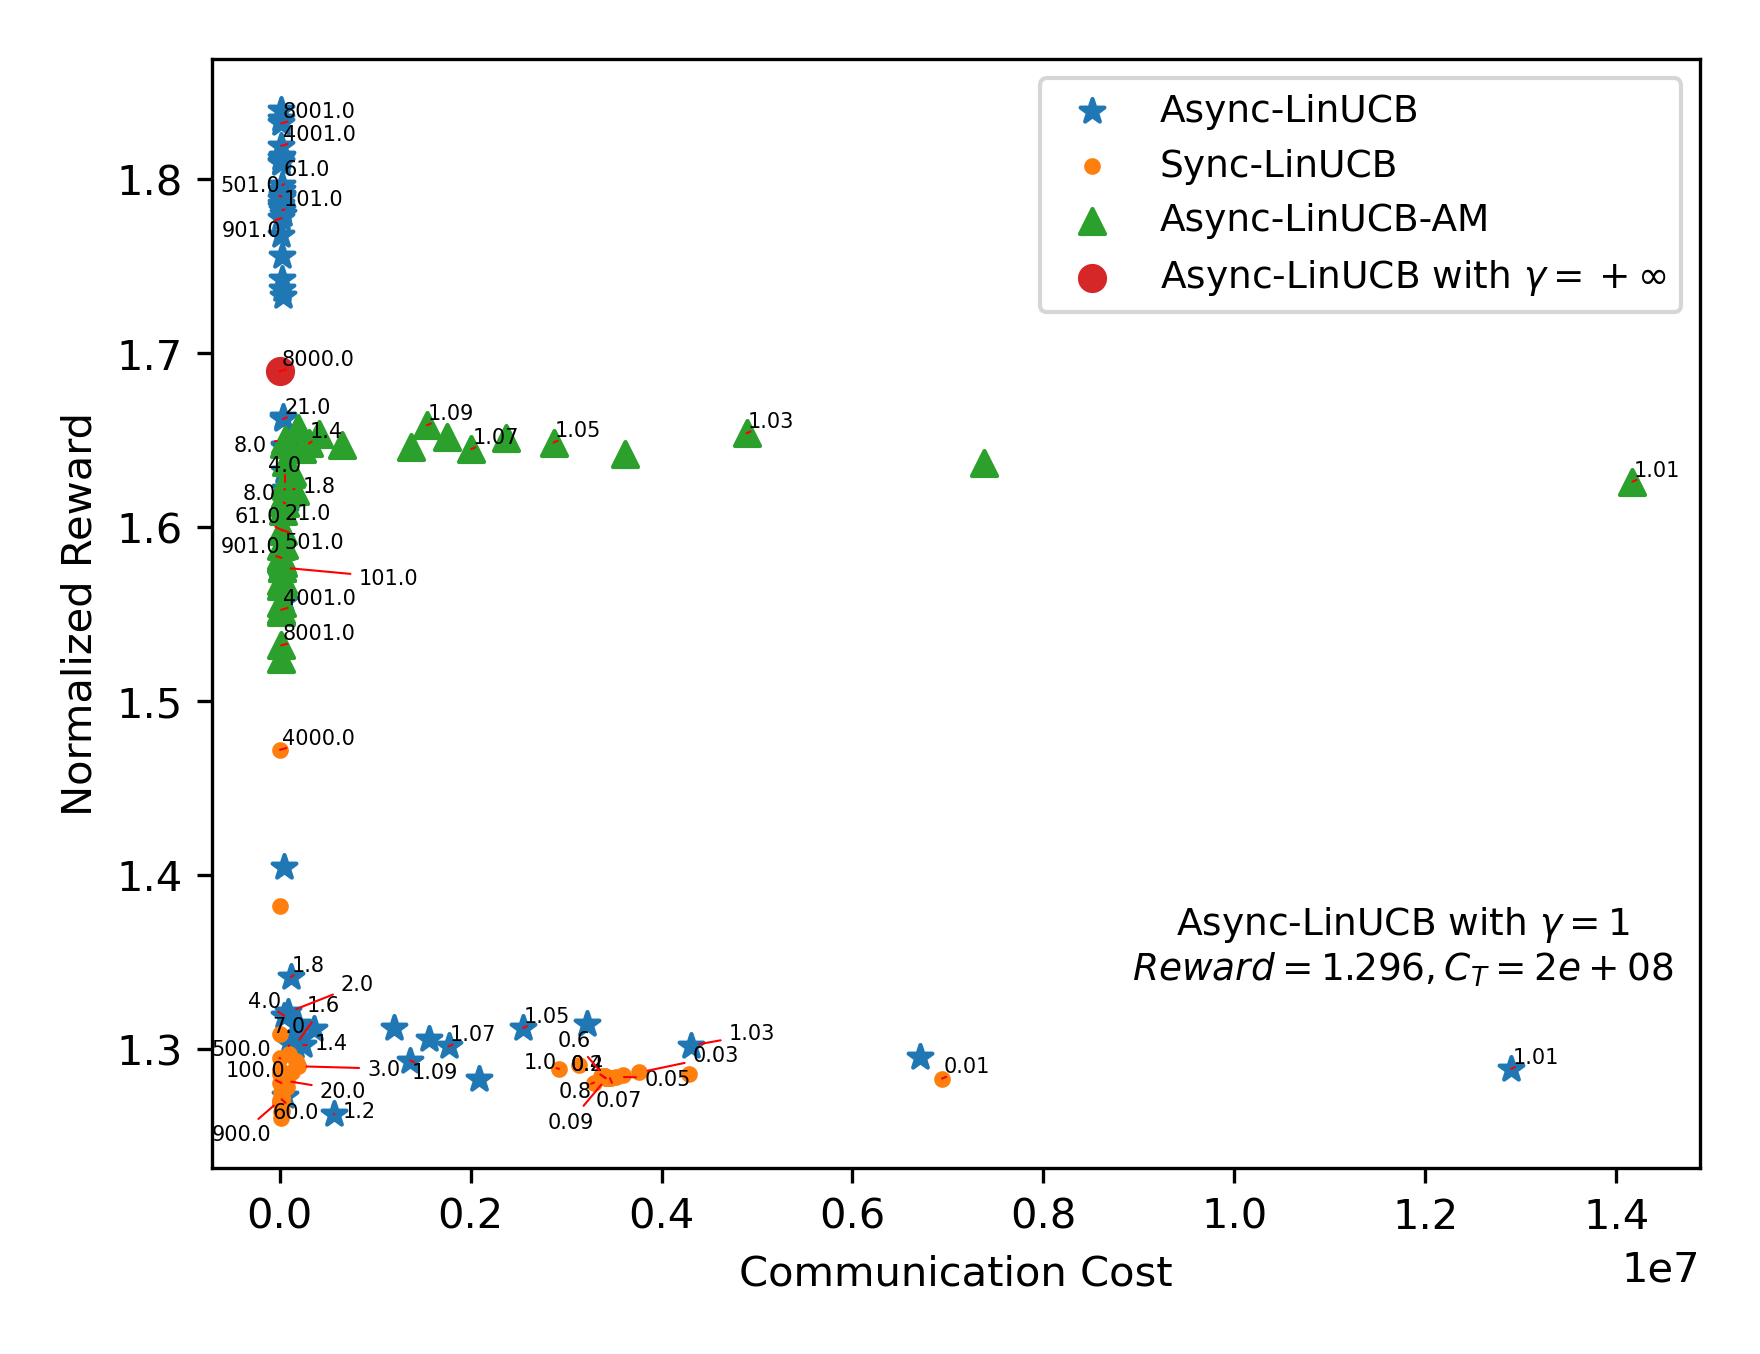
\includegraphics[width=0.32\textwidth]{imgs/regretVScommCost_delicious_noclutter.png}}
% \subfigure[MovieLens ($N=54$)]{\label{fig:f}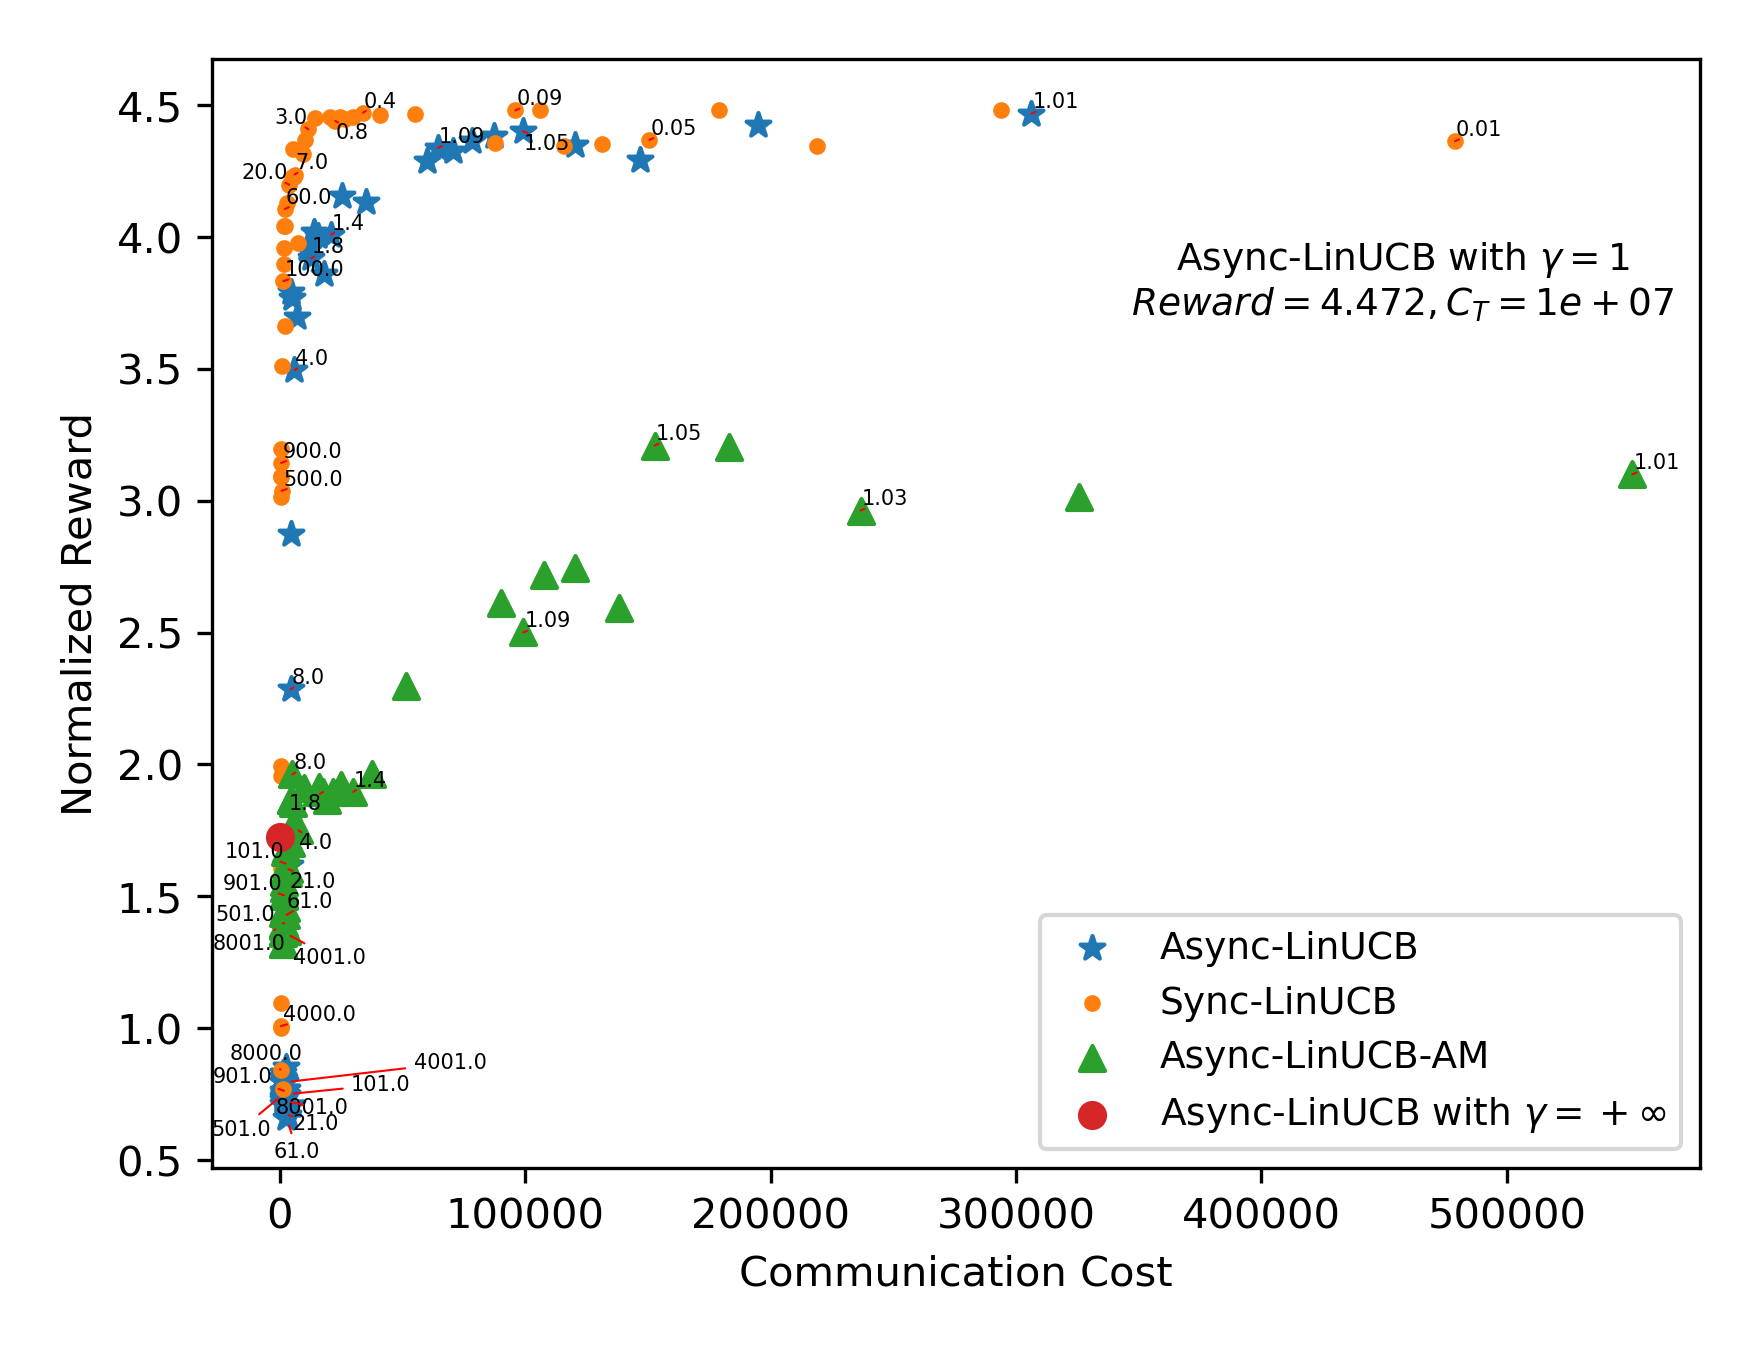
\includegraphics[width=0.32\textwidth]{imgs/regretVScommCost_movielens_noclutter.png}}
% % \vspace{-2.5mm}
% \caption{Experiment results on synthetic and real-world recommendation datasets.}
% % \vspace{-1mm}
% \end{figure*}

% \begin{figure*}[ht]
% \vspace{-2mm}
% \centering
% \begin{tabular}{c c c}
% 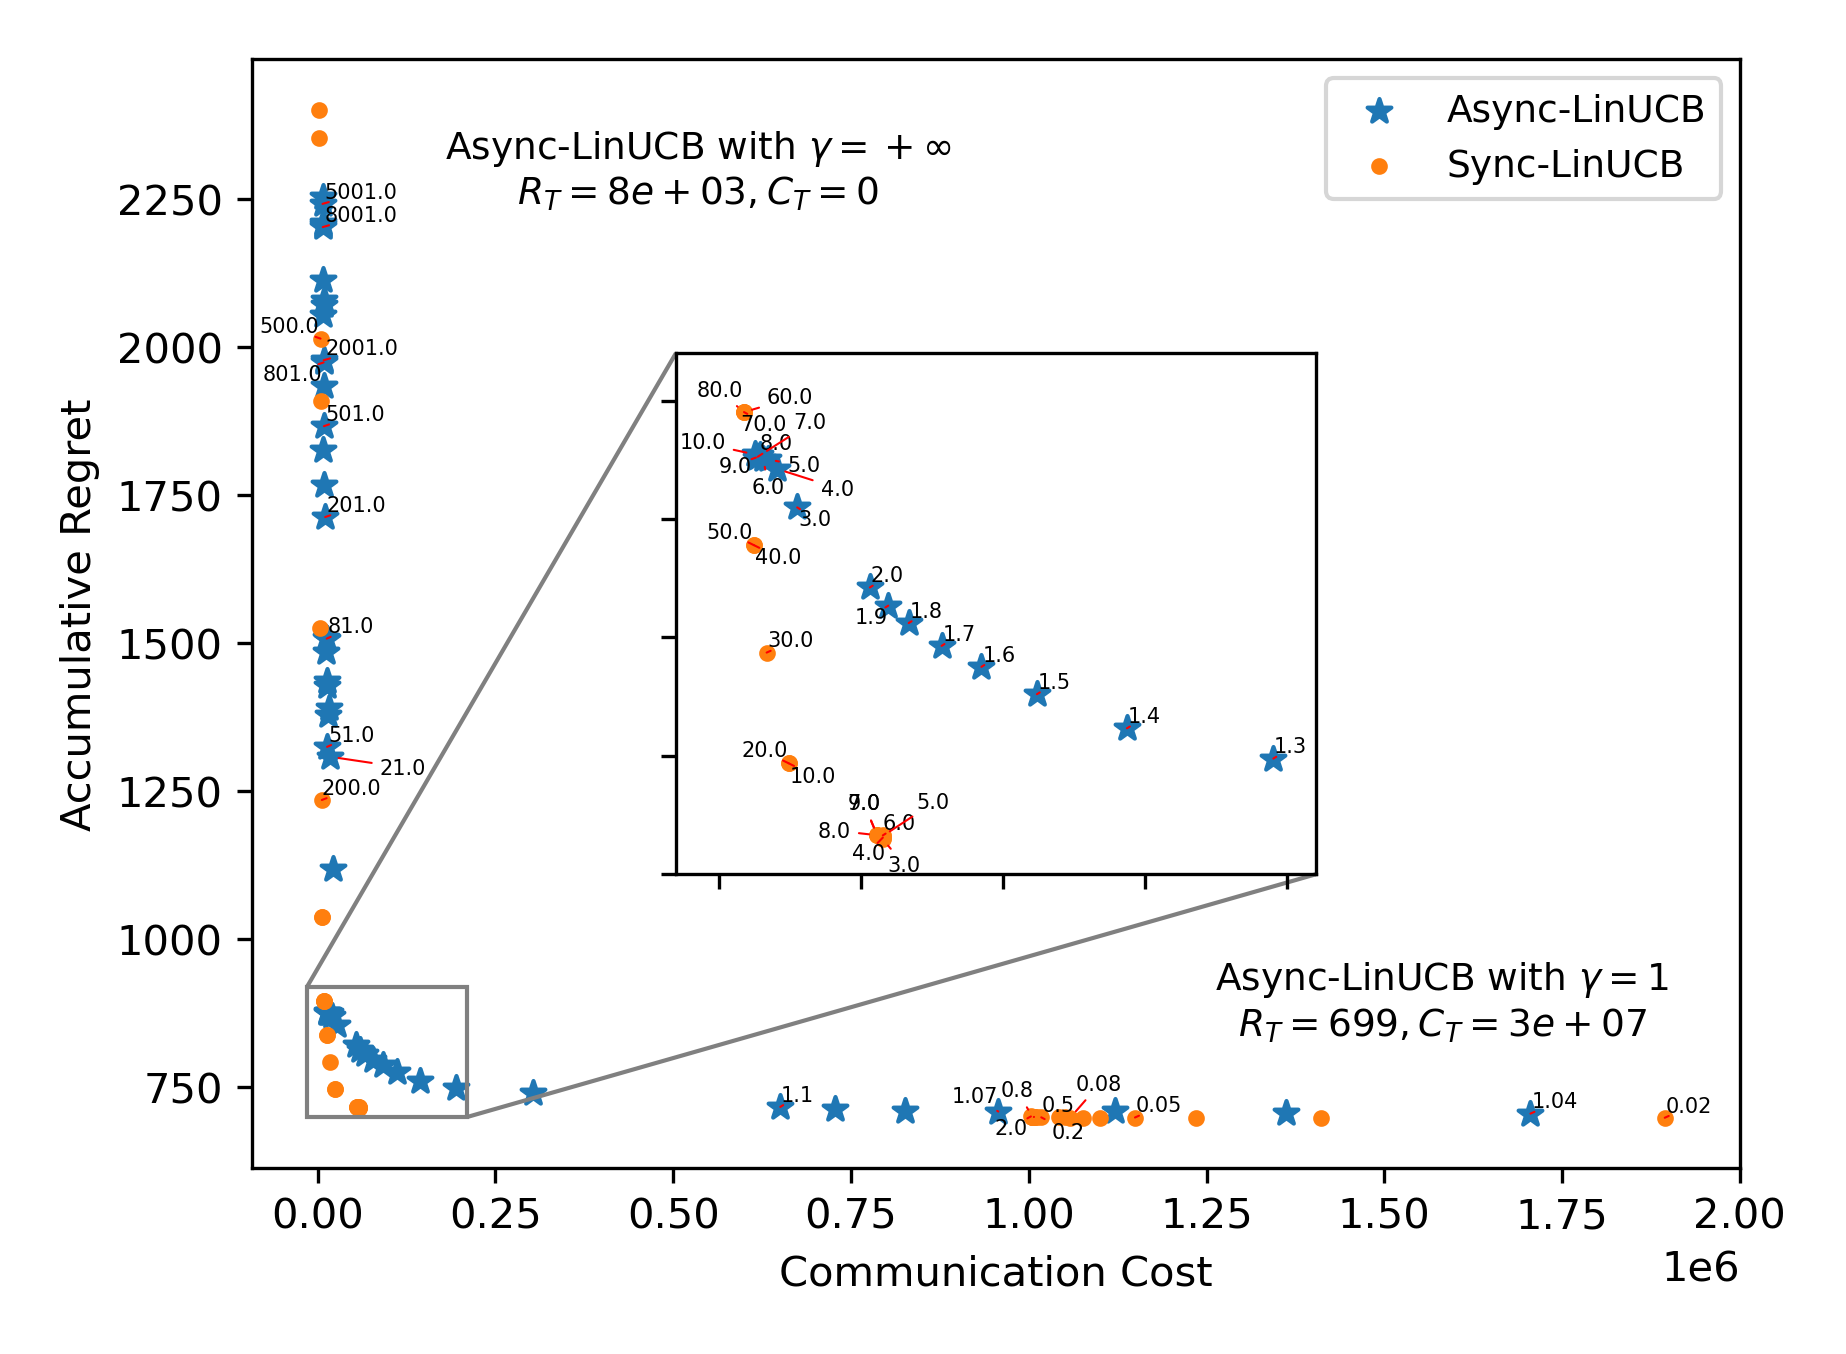
\includegraphics[width=0.32\textwidth]{imgs/regretVScommCost_uniform_noclutter.png} &
% 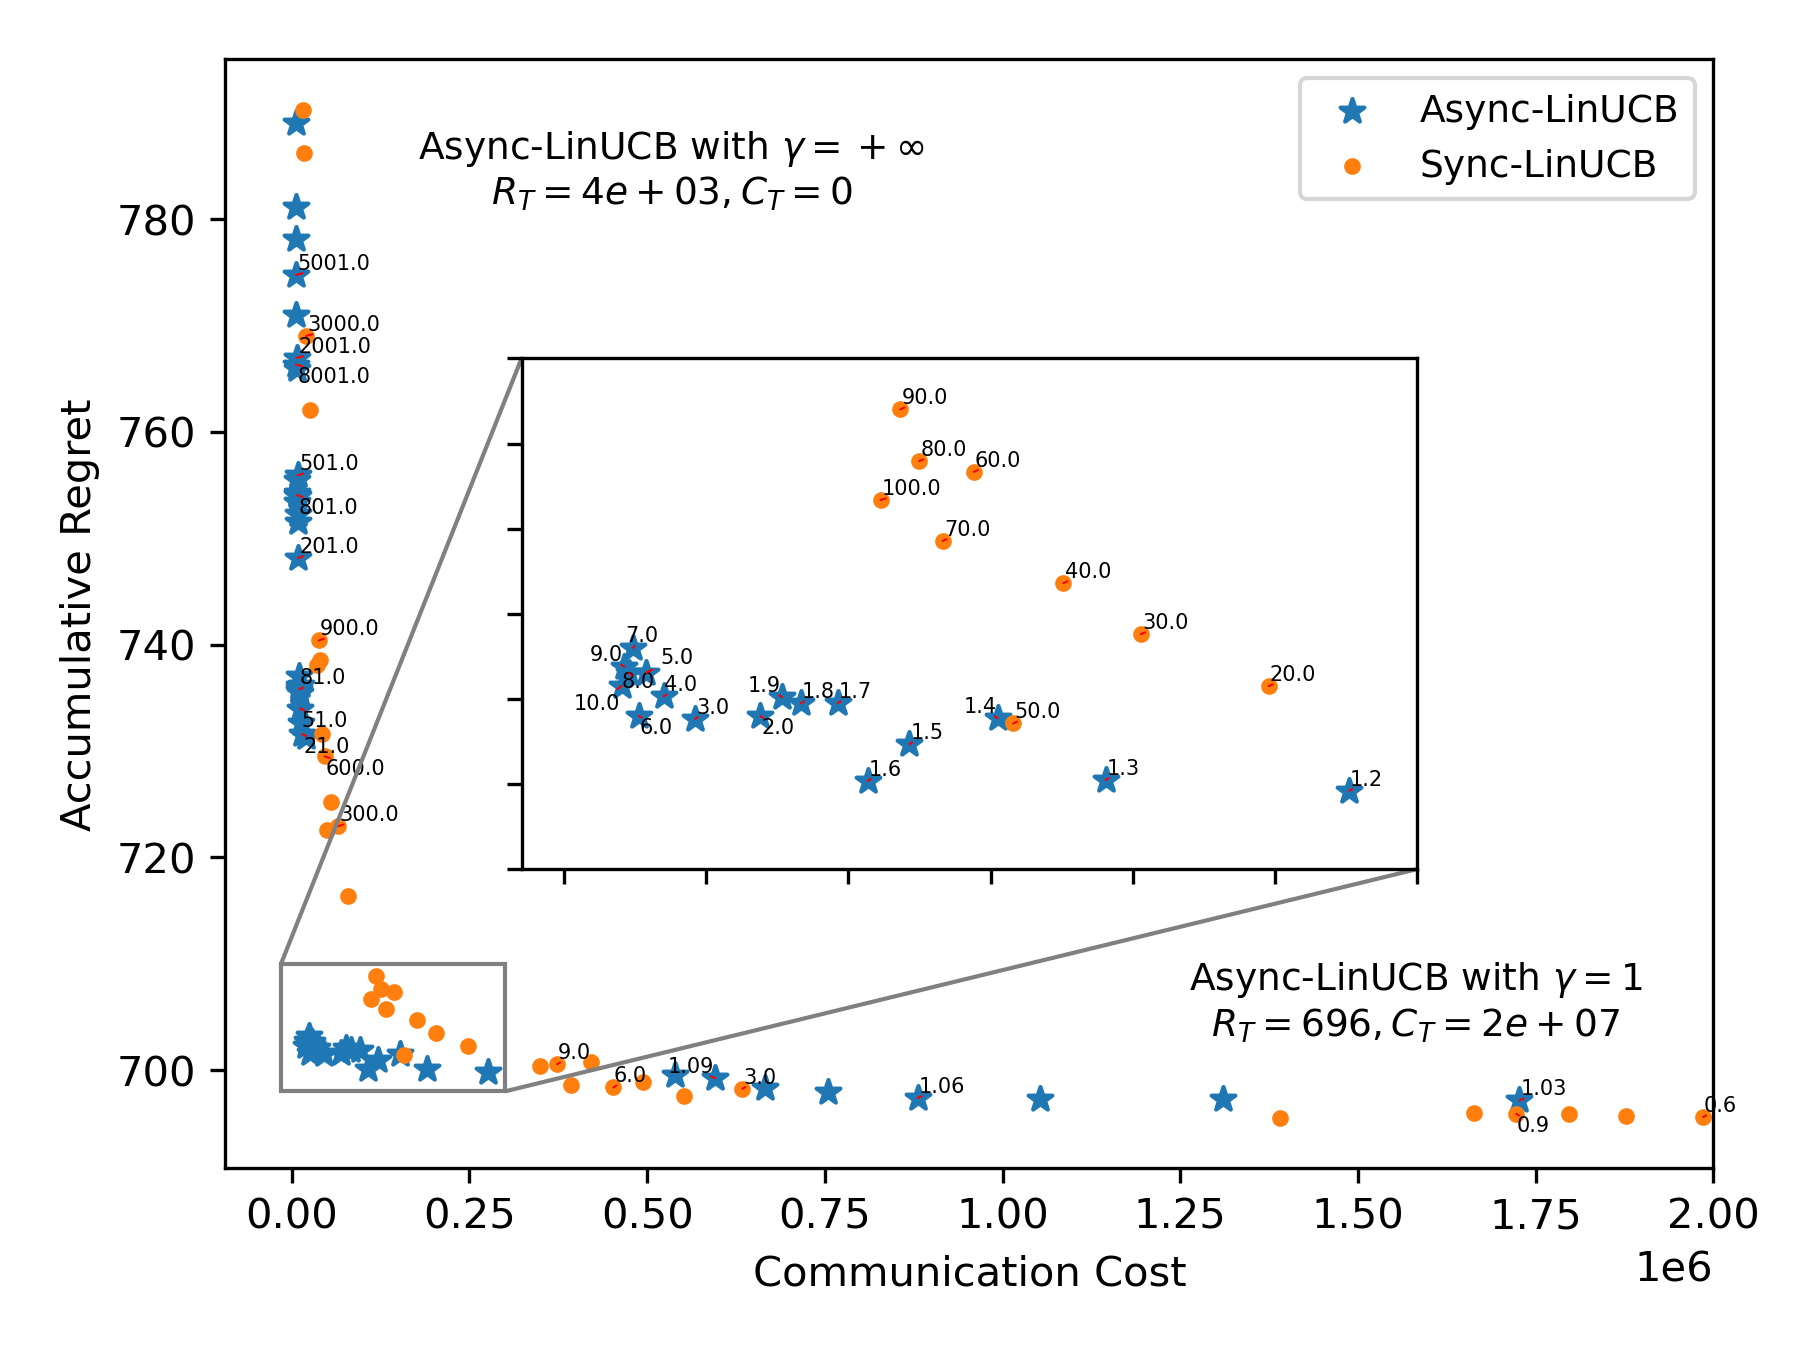
\includegraphics[width=0.32\textwidth]{imgs/regretVScommCost_nonuniform_noclutter.png} &
% 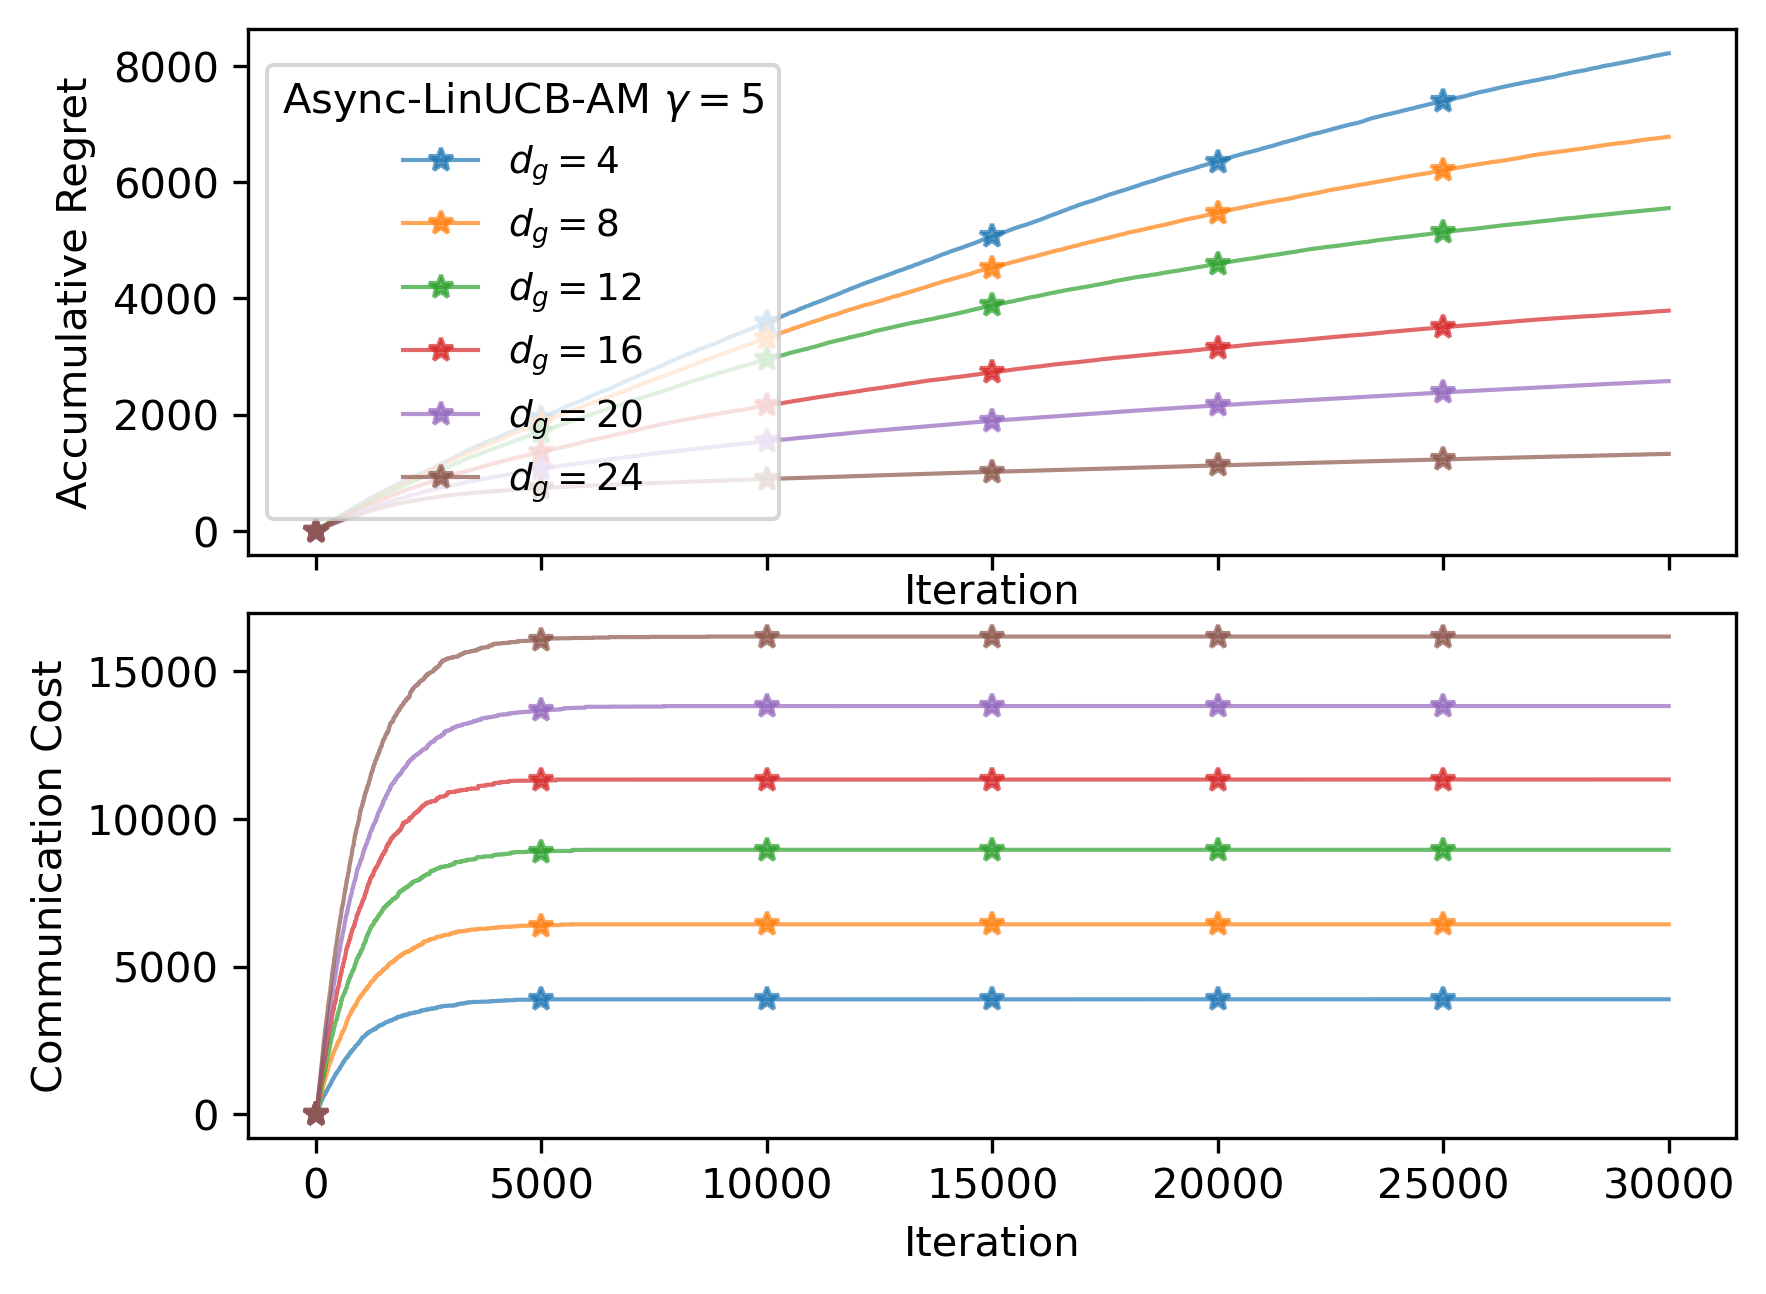
\includegraphics[width=0.31\textwidth]{imgs/sim_hetero_30000.png}\\
% \small (a) Homogeneous (uniform) \normalsize & \small (b) Homogeneous (non-uniform) \normalsize & \small (c) Heterogeneous clients \normalsize\\
% % \includegraphics[width=0.3\textwidth]{imgs/real_lastfm_legend.png} &
% 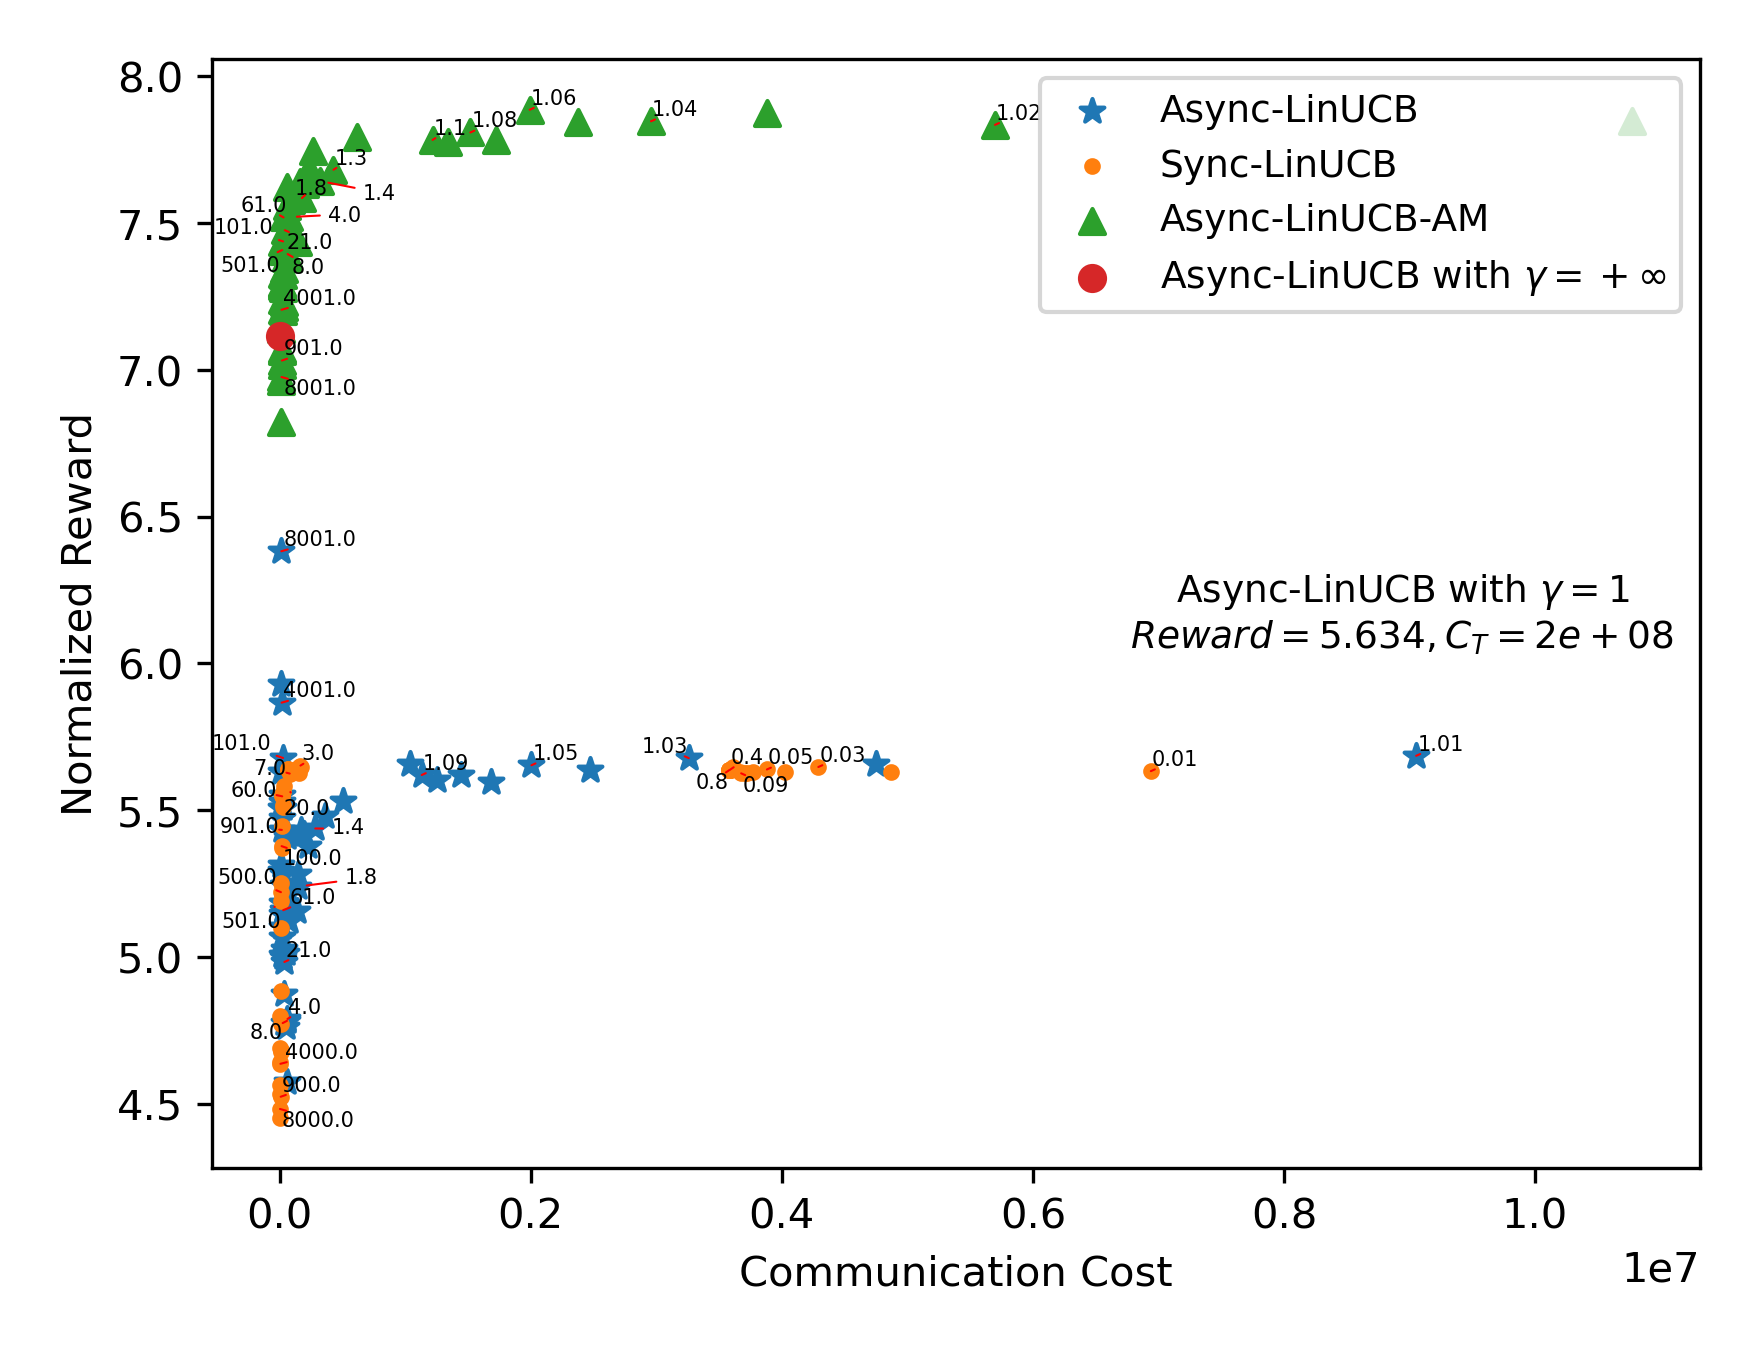
\includegraphics[width=0.31\textwidth]{imgs/regretVScommCost_lastfm_noclutter.png} &
% % \includegraphics[width=0.3\textwidth]{imgs/real_delicious_legend.png} &
% 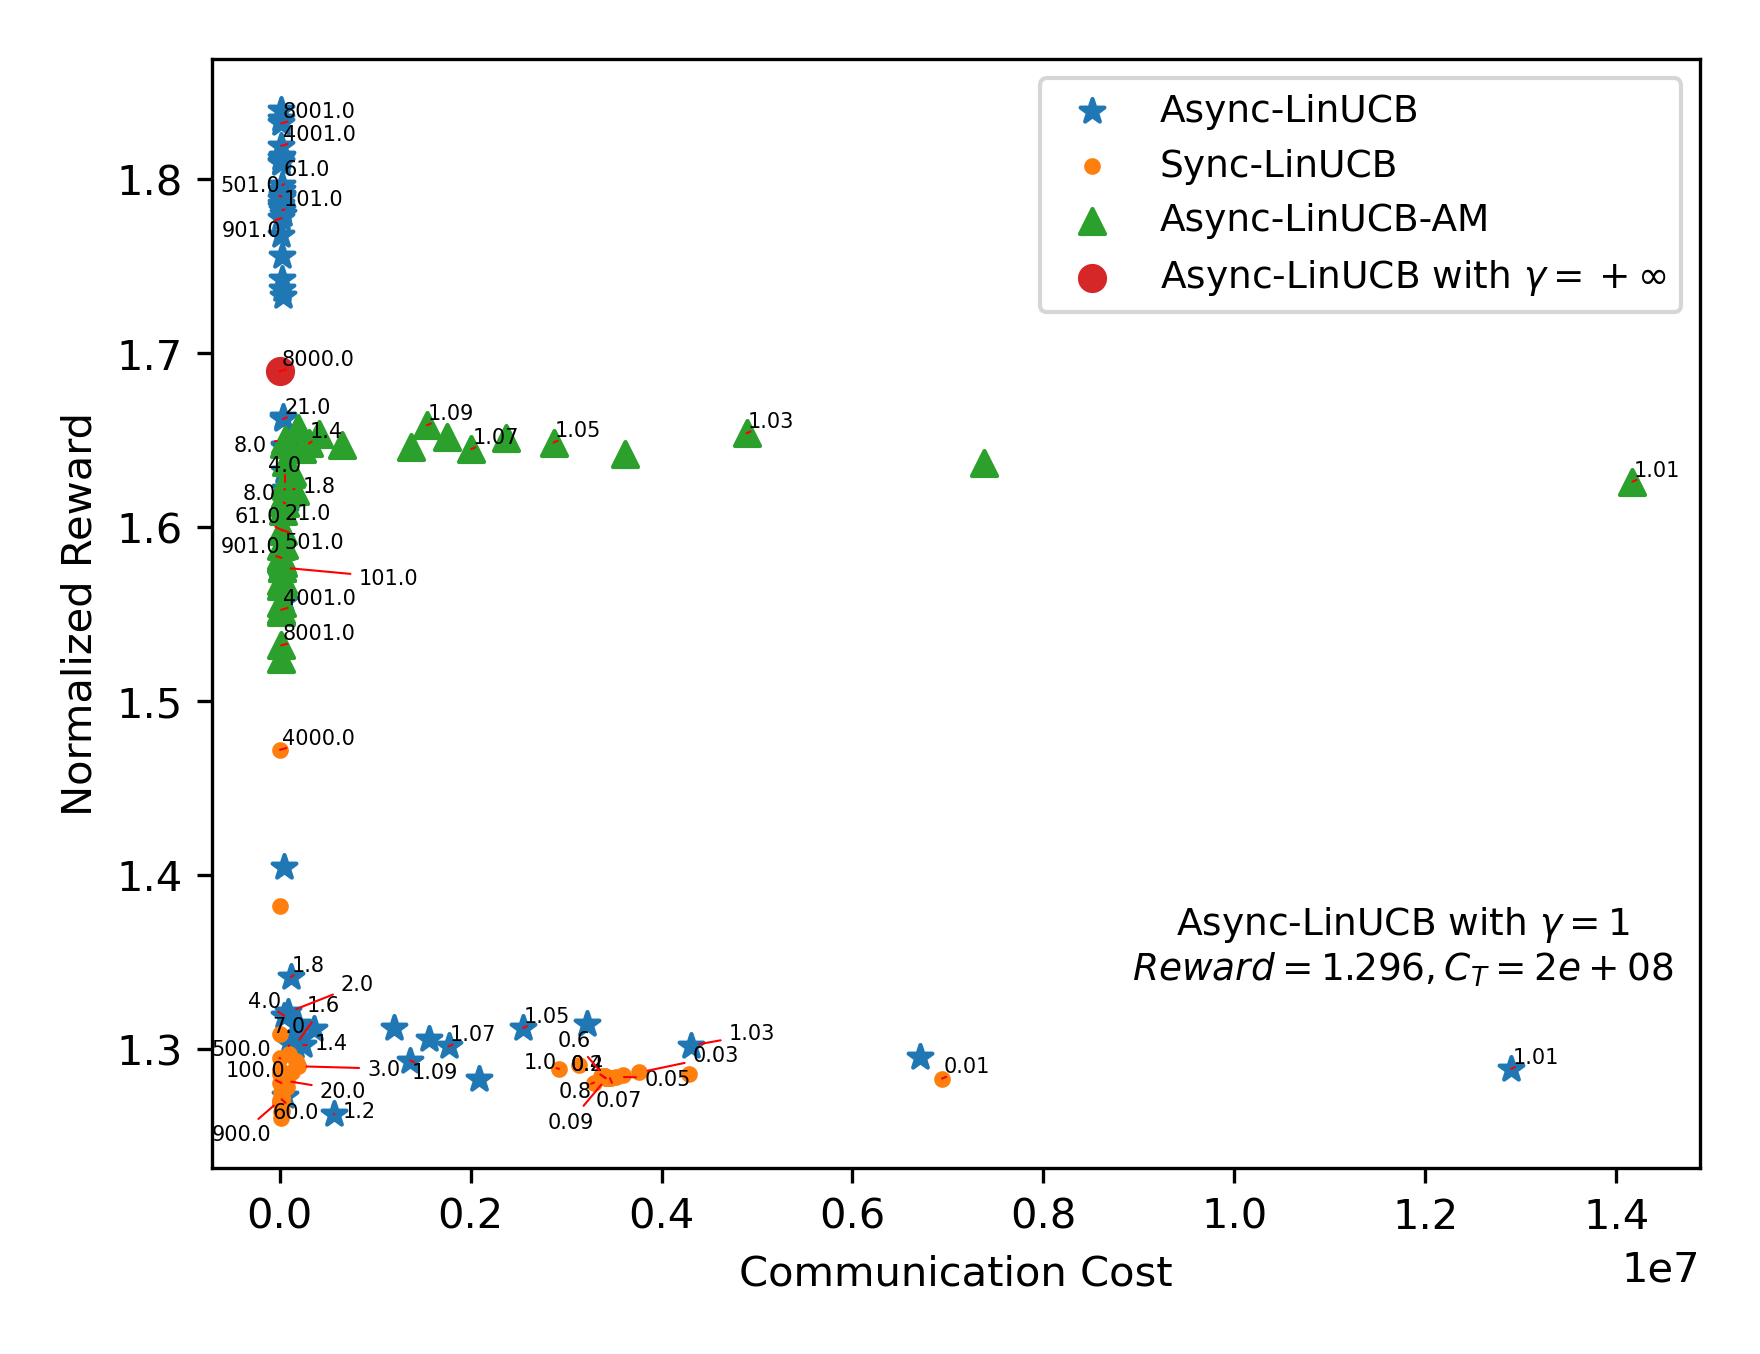
\includegraphics[width=0.31\textwidth]{imgs/regretVScommCost_delicious_noclutter.png} &
% % \includegraphics[width=0.3\textwidth]{imgs/real_movielens_legend.png}\\
% 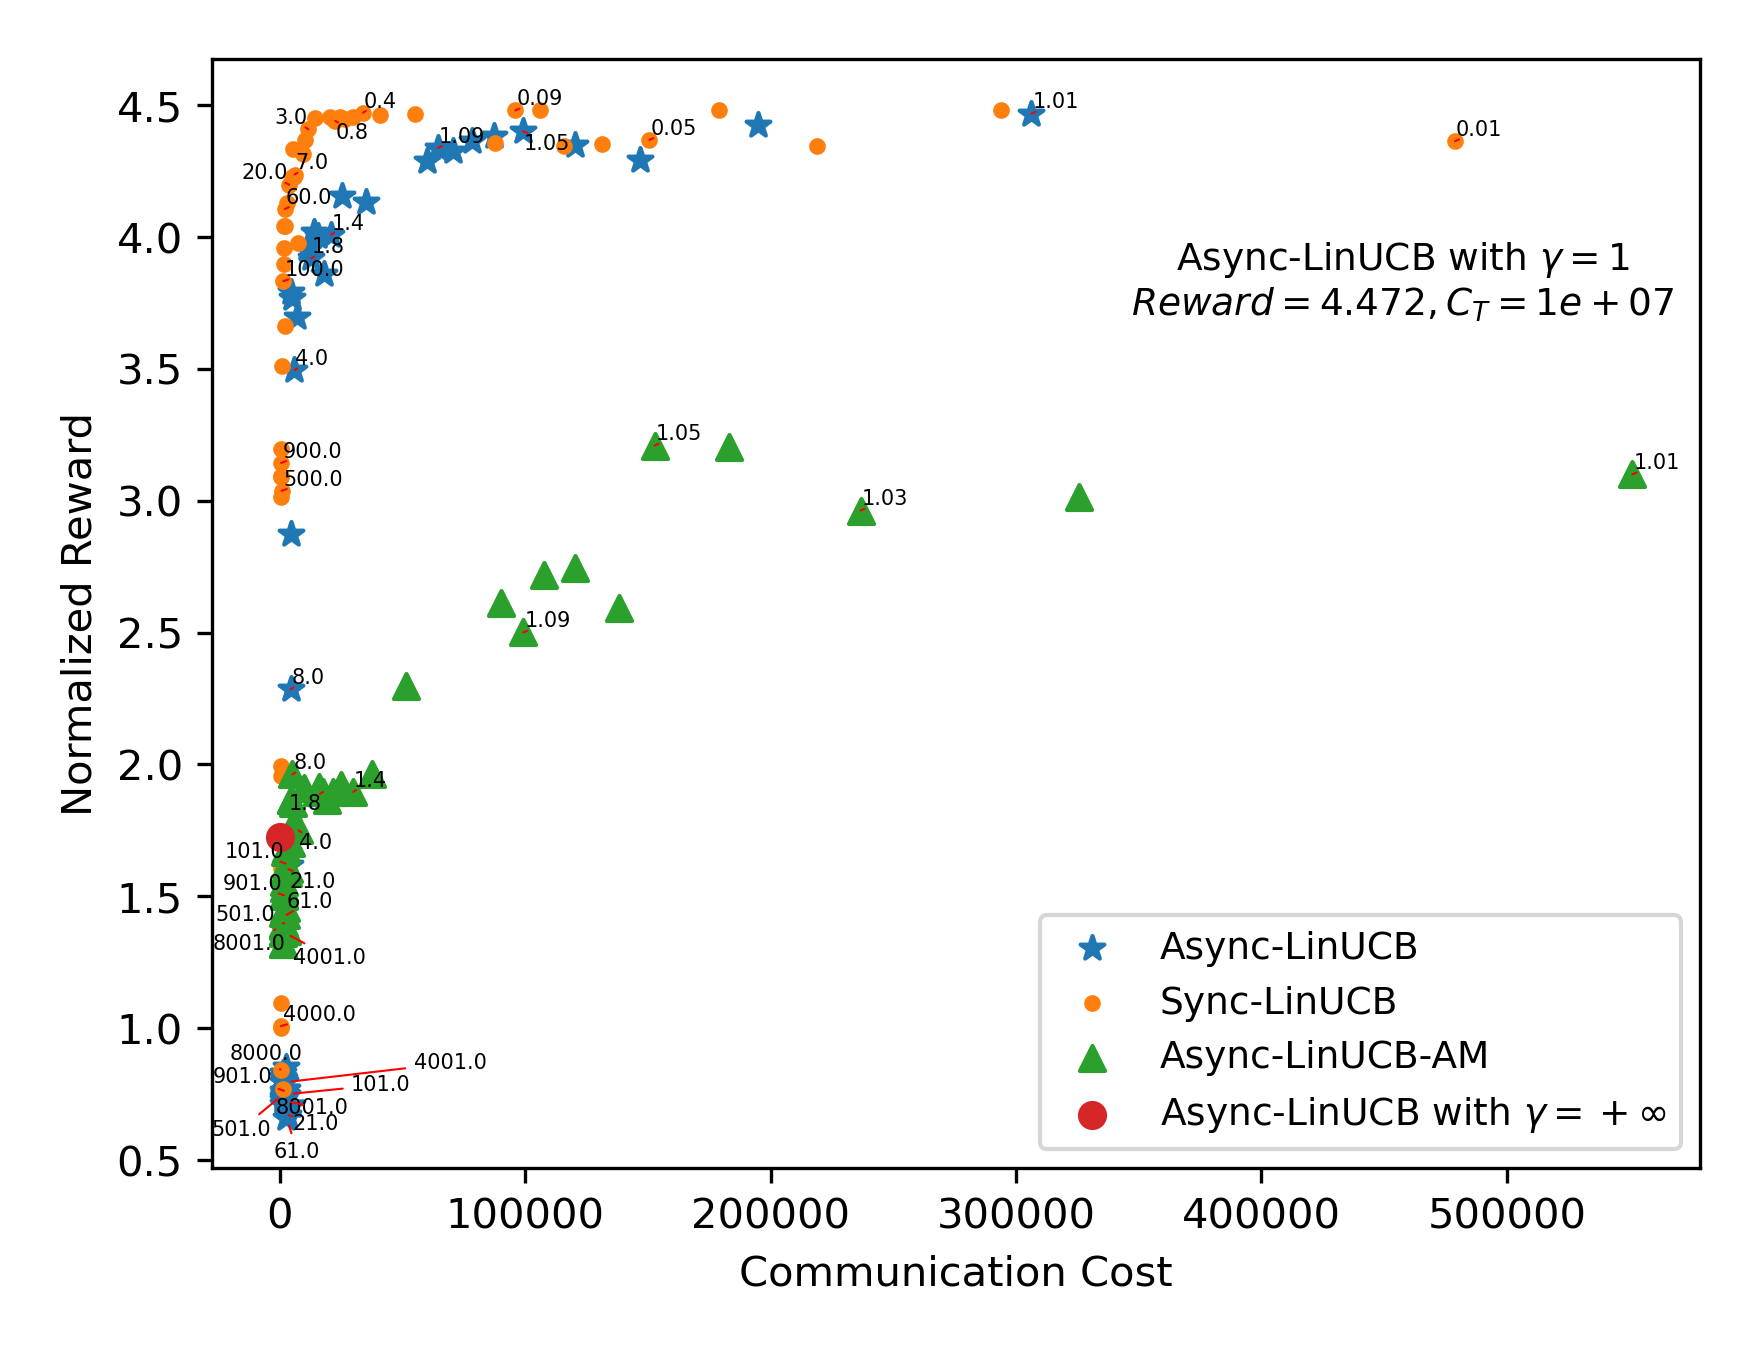
\includegraphics[width=0.31\textwidth]{imgs/regretVScommCost_movielens_noclutter.png}\\
% \multicolumn{1}{c}{\small(d) LastFM ($N=1892$)\normalsize} & \multicolumn{1}{c}{\small(e) Delicious ($N=1867$)\normalsize} & \multicolumn{1}{c}{\small(f) MovieLens ($N=54$)\normalsize}
% \end{tabular}
% \caption{Experiment results on synthetic and real-world recommendation datasets.} \label{fig:exp_result}
% % \vspace{-2mm}
% \end{figure*}

% \begin{figure*}[ht]
% \centering
% \begin{tabular}{c c c}
% \includegraphics[width=5.2cm]{imgs/real_lastfm.png} &
% \includegraphics[width=5.2cm]{imgs/real_delicious.png} &
% \includegraphics[width=5.2cm]{imgs/real_movielens.png} \\
% \small (a) LastFM ($T=96733, N=1892$)  & (b) Delicious ($T=104799,N=1867$) & \small (b) MovieLens ($T=214729,N=54$)
% \normalsize
% \end{tabular}
% \caption{Normalized accumulative reward and communication cost on real-world datasets.} \label{fig:realworld}
% \end{figure*}



% \begin{figure*}[ht]
% \centering
% \begin{tabular}{c c c}
%  \multicolumn{1}{c}{\includegraphics[width=0.3\textwidth]{imgs/sim_homo_50000_marker_repeat_legend.png}} &
%  \multicolumn{1}{c}{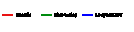
\includegraphics[width=3cm]{imgs/legend.png}} &
%  \multicolumn{1}{c}{\includegraphics[width=0.3\textwidth]{imgs/sim_hetero_50000_marker_repeat_legend.png}}\\
% \multicolumn{1}{c}{\small(a) Homogeneous clients ($T=50000,N=1000$)\normalsize} &
% % & \multicolumn{2}{c}{$\quad $} 
% & \multicolumn{1}{c}{ \small(b) Heterogeneous clients ($T=50000,N=1000$)\normalsize} \\
% \multicolumn{1}{c}{\includegraphics[width=5.3cm]{imgs/real_lastfm.png}} & \multicolumn{1}{c}{\includegraphics[width=5.4cm]{imgs/real_delicious.png}} & \multicolumn{1}{c}{\includegraphics[width=5.3cm]{imgs/real_movielens.png}} \\
% \multicolumn{1}{c}{\small(c) LastFM ($T=96733, N=1892$)\normalsize} & \multicolumn{1}{c}{\small(d) Delicious ($T=104799,N=1867$)\normalsize} & \multicolumn{1}{c}{\small(e) MovieLens ($T=214729,N=54$)\normalsize} \\
% \end{tabular}
% \caption{Experiment results on synthetic and real-world recommendation datasets.} \label{fig:exp_result}
% \end{figure*}

\section{Experiments}\label{sec:exp}
We performed extensive empirical evaluations of \modelone{} and \modeltwo{} on both synthetic and real-world datasets (we set $\gamma_{U}=\gamma_{D}=\gamma$ in all experiments), and included \modelbaseline{} \citep{wang2019distributed} as baseline. 
% Due to the space limit, we provide a brief summary of the experiment setup and results. Detailed descriptions and discussions are presented in the appendix.
\subsection{Experiments on Synthetic Dataset}
To validate our theoretical analysis in Section \ref{subsec:async_LinUCB} and Section \ref{subsec:async_LinUCB_AM}, two sets of simulation experiments were conducted.
We first conducted simulation experiment in homogeneous client setting to
% compare how well the algorithms can balance regret $R_{T}$ and communication cost $C_{T}$ under uniform and non-uniform client distributions, as well as 
validate our theoretical comparison between \modelone{} and \modelbaseline{} (see Section \ref{subsec:async_LinUCB} and Section \ref{sec:tb_theretical} in appendix), i.e., how well the algorithms balance regret $R_{T}$ and communication cost $C_{T}$ under uniform and non-uniform client distributions. Then we conducted simulation experiment in heterogeneous setting to validate our regret upper bound for \modeltwo{} (see Section \ref{subsec:async_LinUCB_AM}), i.e., how the portion of global components $\frac{d_{g}}{d_{g}+d_{i}}$ in the bandit parameter affects the regret of \modeltwo{}.
\subsubsection{Synthetic dataset.} We simulated the federated linear bandit problem setting in Section \ref{subsec:problem_formulation}, with $T=30000, N=1000$, and $\cA_{t}$ ($K=25$) uniformly sampled from a $\ell_2$ ball.
% is sampled from a pool of $1000$ randomly generated arms. 
% Two sets of simulation experiments were performed, with 
(1) Homogeneous clients: 
To compare how the algorithms balance $R_{T}$ and $C_{T}$ under uniform ($P(i_{t}=i)=\frac{1}{N},\forall i,t$) and non-uniform client distributions ($P(i_{t})$ is an arbitrary point on probability simplex), we fixed $d=25$, and ran \modelone{} and \modelbaseline{} with a large range of threshold values (logarithmically spaced between $10^{-2}$ and $10^{3}$).
% To compare algorithms' regret and communication cost under different trade-off settings over time, we fix $d=25$, $L=S=1$, and run \modelone{} with $\gamma \in \{1,2,5,8,+\infty\}$, \modelbaseline{} with threshold $D \in \{\frac{T}{d N^{2} \log{T}}, \frac{T}{d N^{1.5} \log{T}}\}$ (see Remark \ref{rmk:regret}) with both uniformly and non-uniformly sampled clients.
(2) Heterogeneous clients: To see how $R_{T}$ and $C_{T}$ of \modeltwo{} changes as the portion of global components change, we set the local components for all clients to have equal dimension, i.e., $d_{i}=d_{l},\forall i \in [N]$, fixed $d_{g}+d_{l}=25$, $\forall i\in [N]$, and then ran \modeltwo{} (with $\gamma=5$) under varying $d_{g} \in \{4,8,12,16,20,24\}$.

\subsubsection{Experiment results.}
Experiment results (averaged over $10$ runs) on synthetic dataset are shown in Figure
% \ref{fig:exp_result}(a)-(c):
\ref{fig:a}-\ref{fig:c}. 
Note that in the scatter plots, 
% the x-axis is the total communication cost at iteration $T$ and the y-axis is the corresponding accumulative regret/reward at iteration $T$. 
each dot denotes the cumulative communication cost (x-axis) and regret (y-axis) that an algorithm (\modelone{} or \modelbaseline{}) with certain threshold value (labeled next to the dot) has obtained at iteration $T$.

\begin{figure}
\centering     %%% not \center
\subfigure[Homogeneous (uniform client distribution)]{\label{fig:a}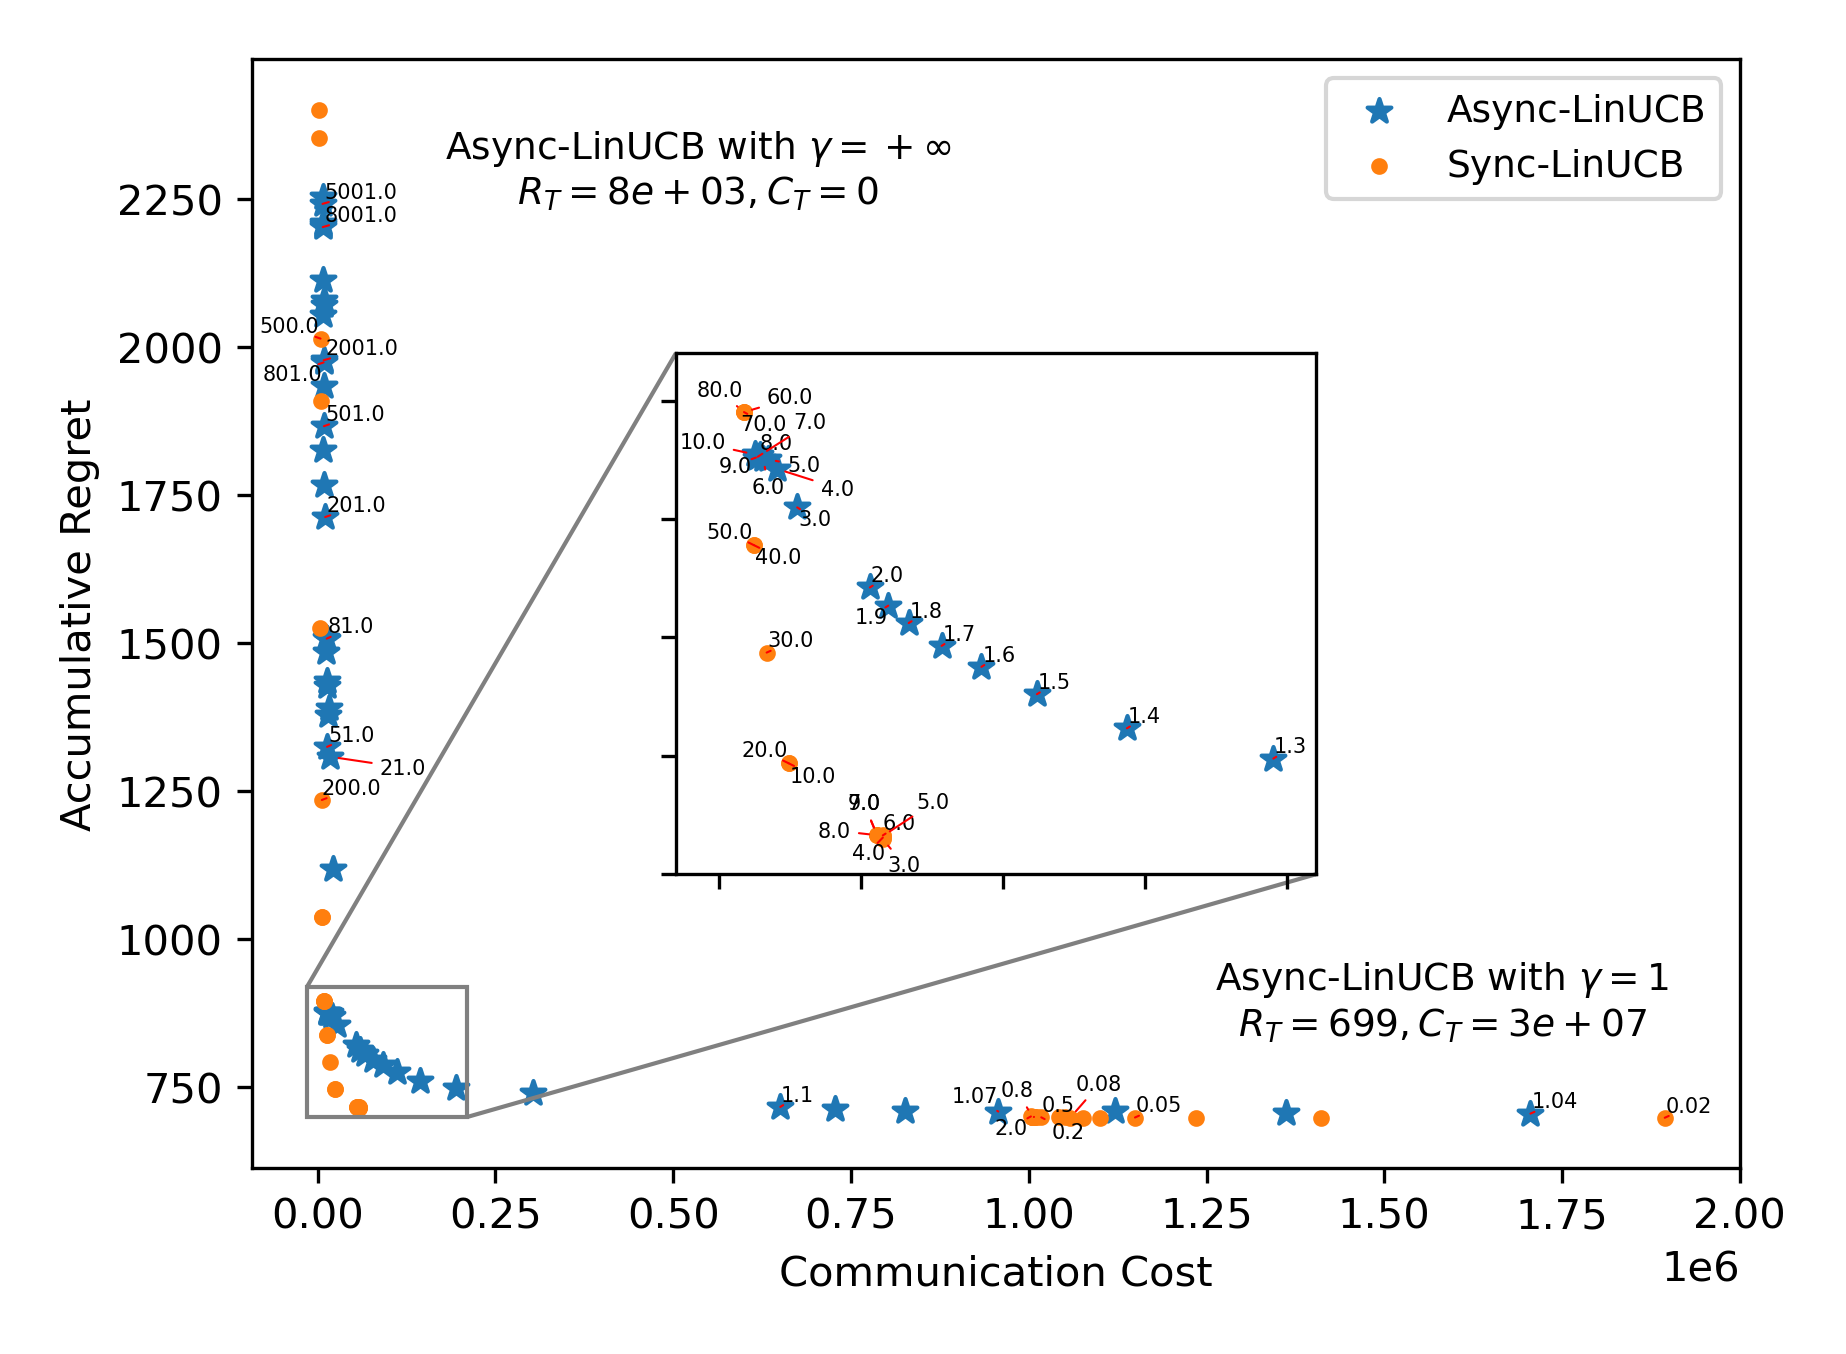
\includegraphics[width=0.55\textwidth]{imgs/regretVScommCost_uniform_noclutter.png}}
\vspace{-1mm}
\subfigure[Homogeneous (non-uniform client distribution)]{\label{fig:b}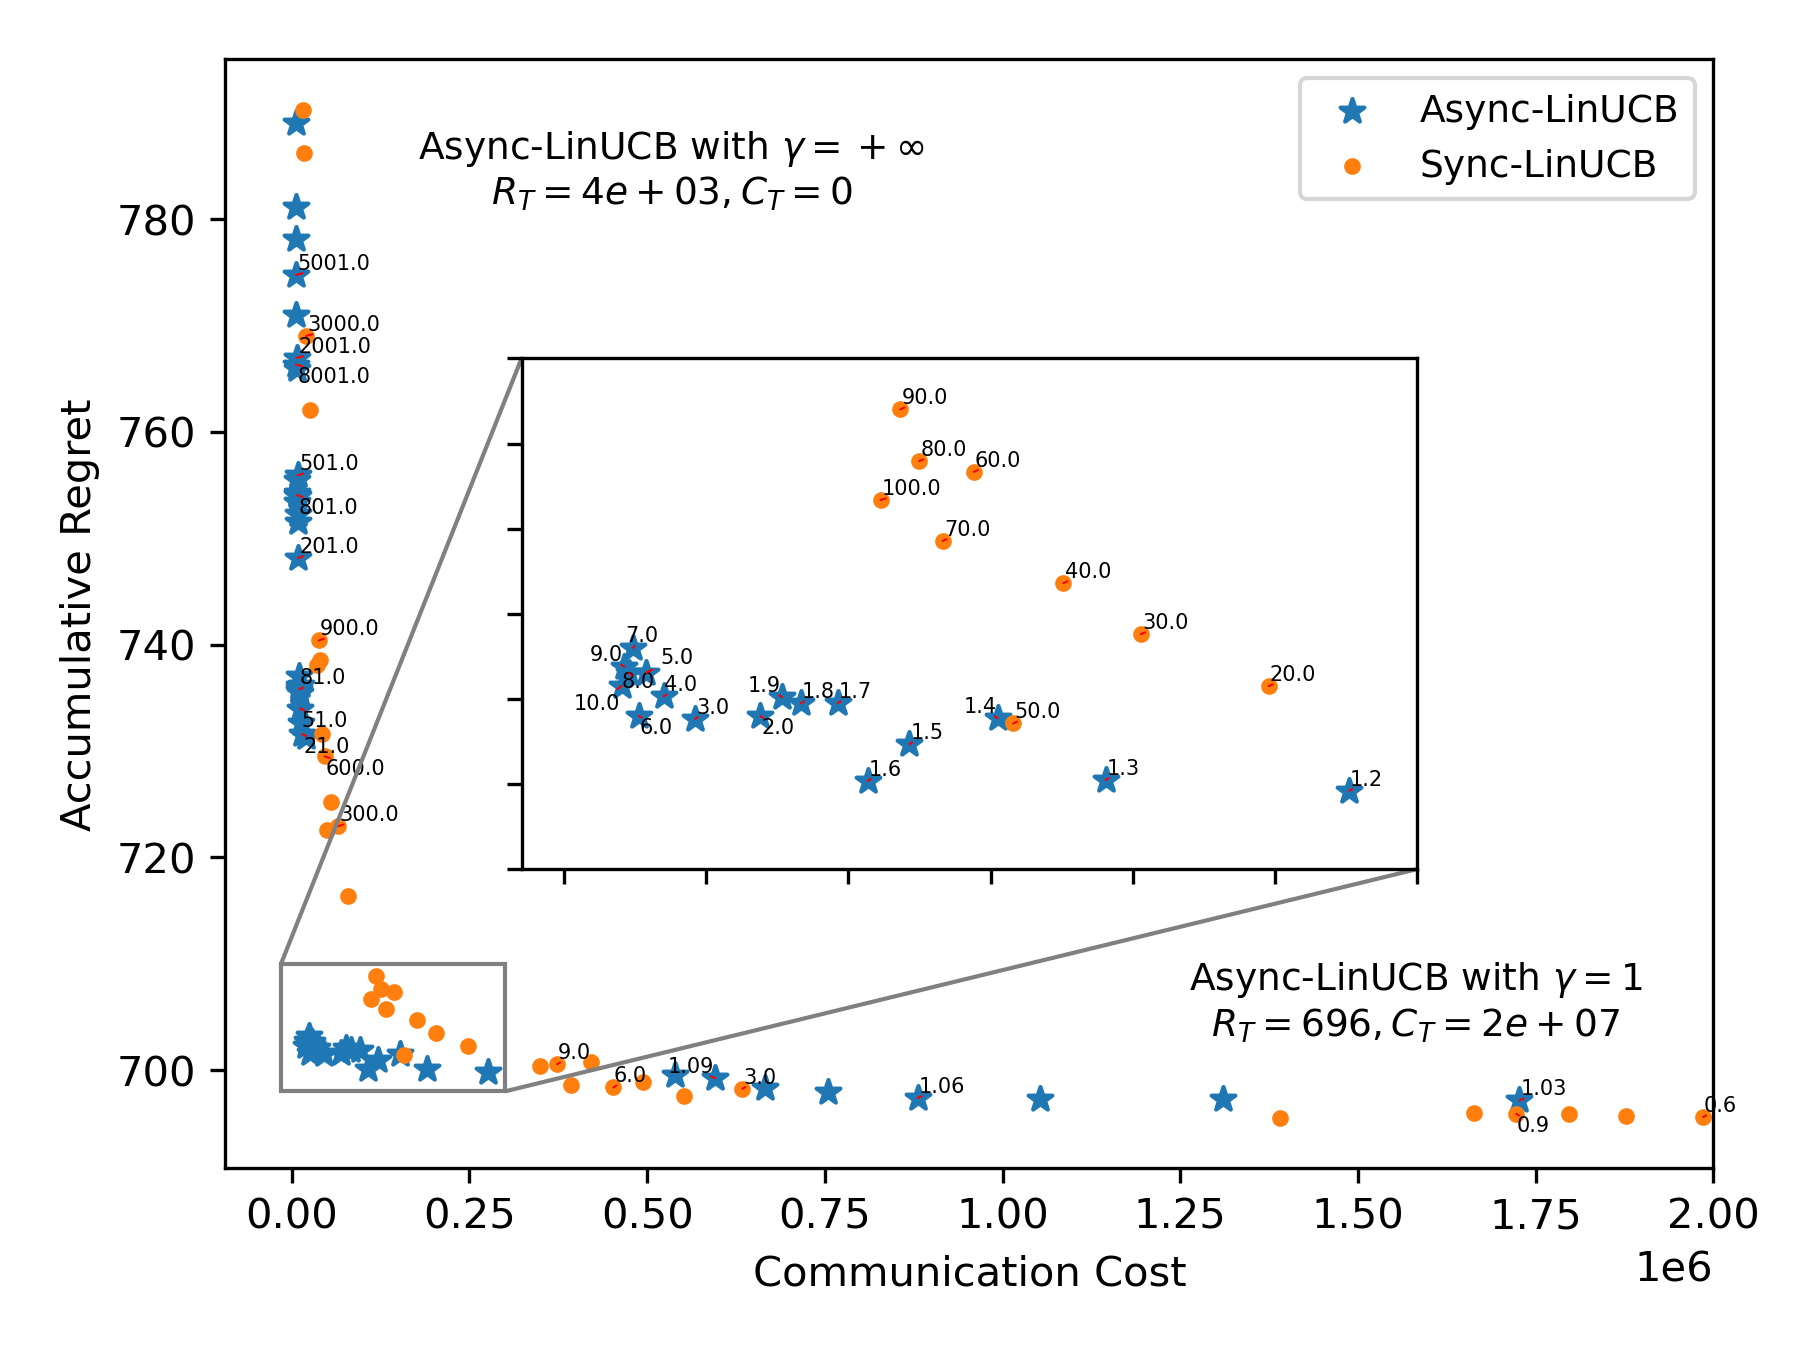
\includegraphics[width=0.55\textwidth]{imgs/regretVScommCost_nonuniform_noclutter.png}}
\vspace{-1mm}
%\medskip
\subfigure[Heterogeneous clients]{\label{fig:c}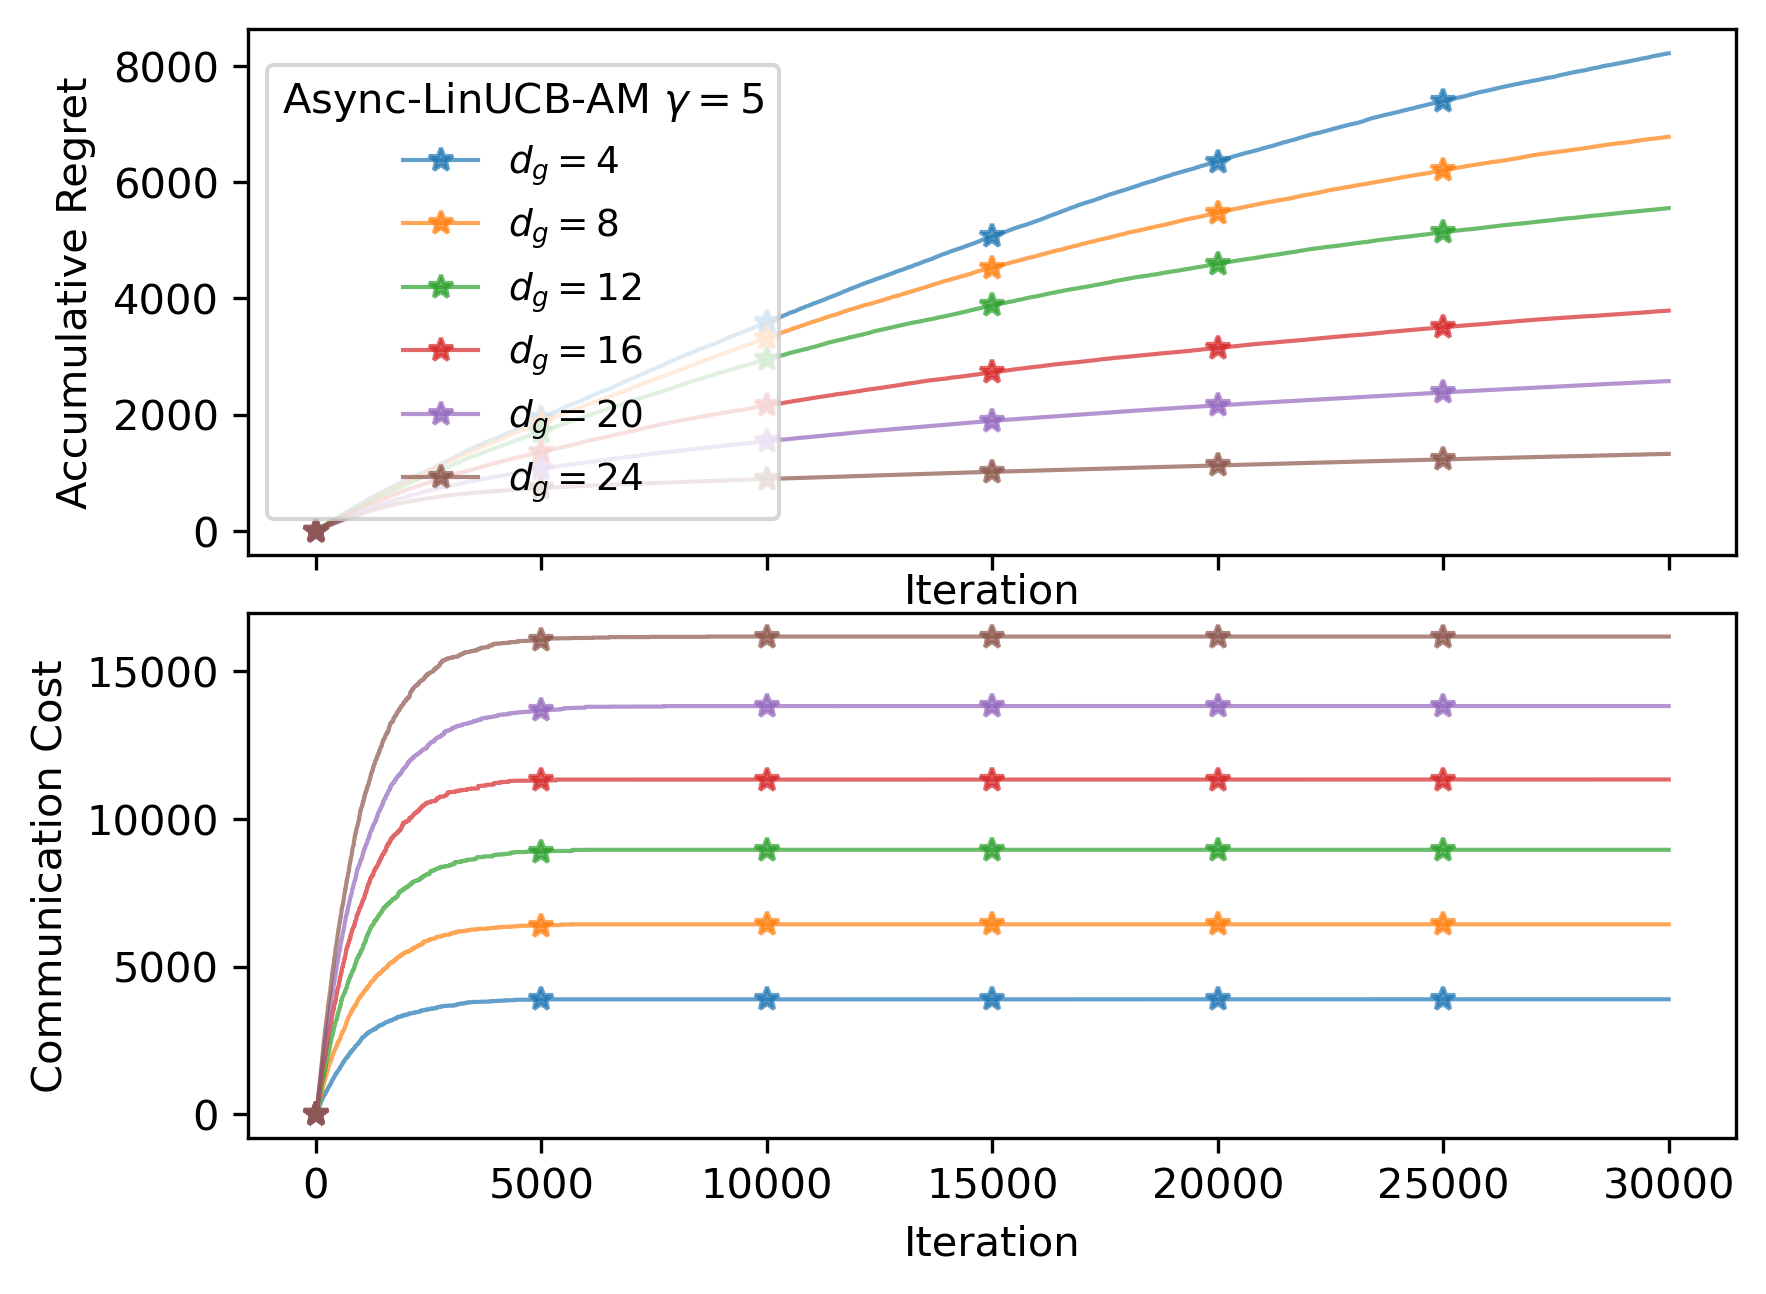
\includegraphics[width=0.55\textwidth]{imgs/sim_hetero_30000.png}}
% \vspace{-1mm}
% \subfigure[LastFM ($N=1892$)]{\label{fig:d}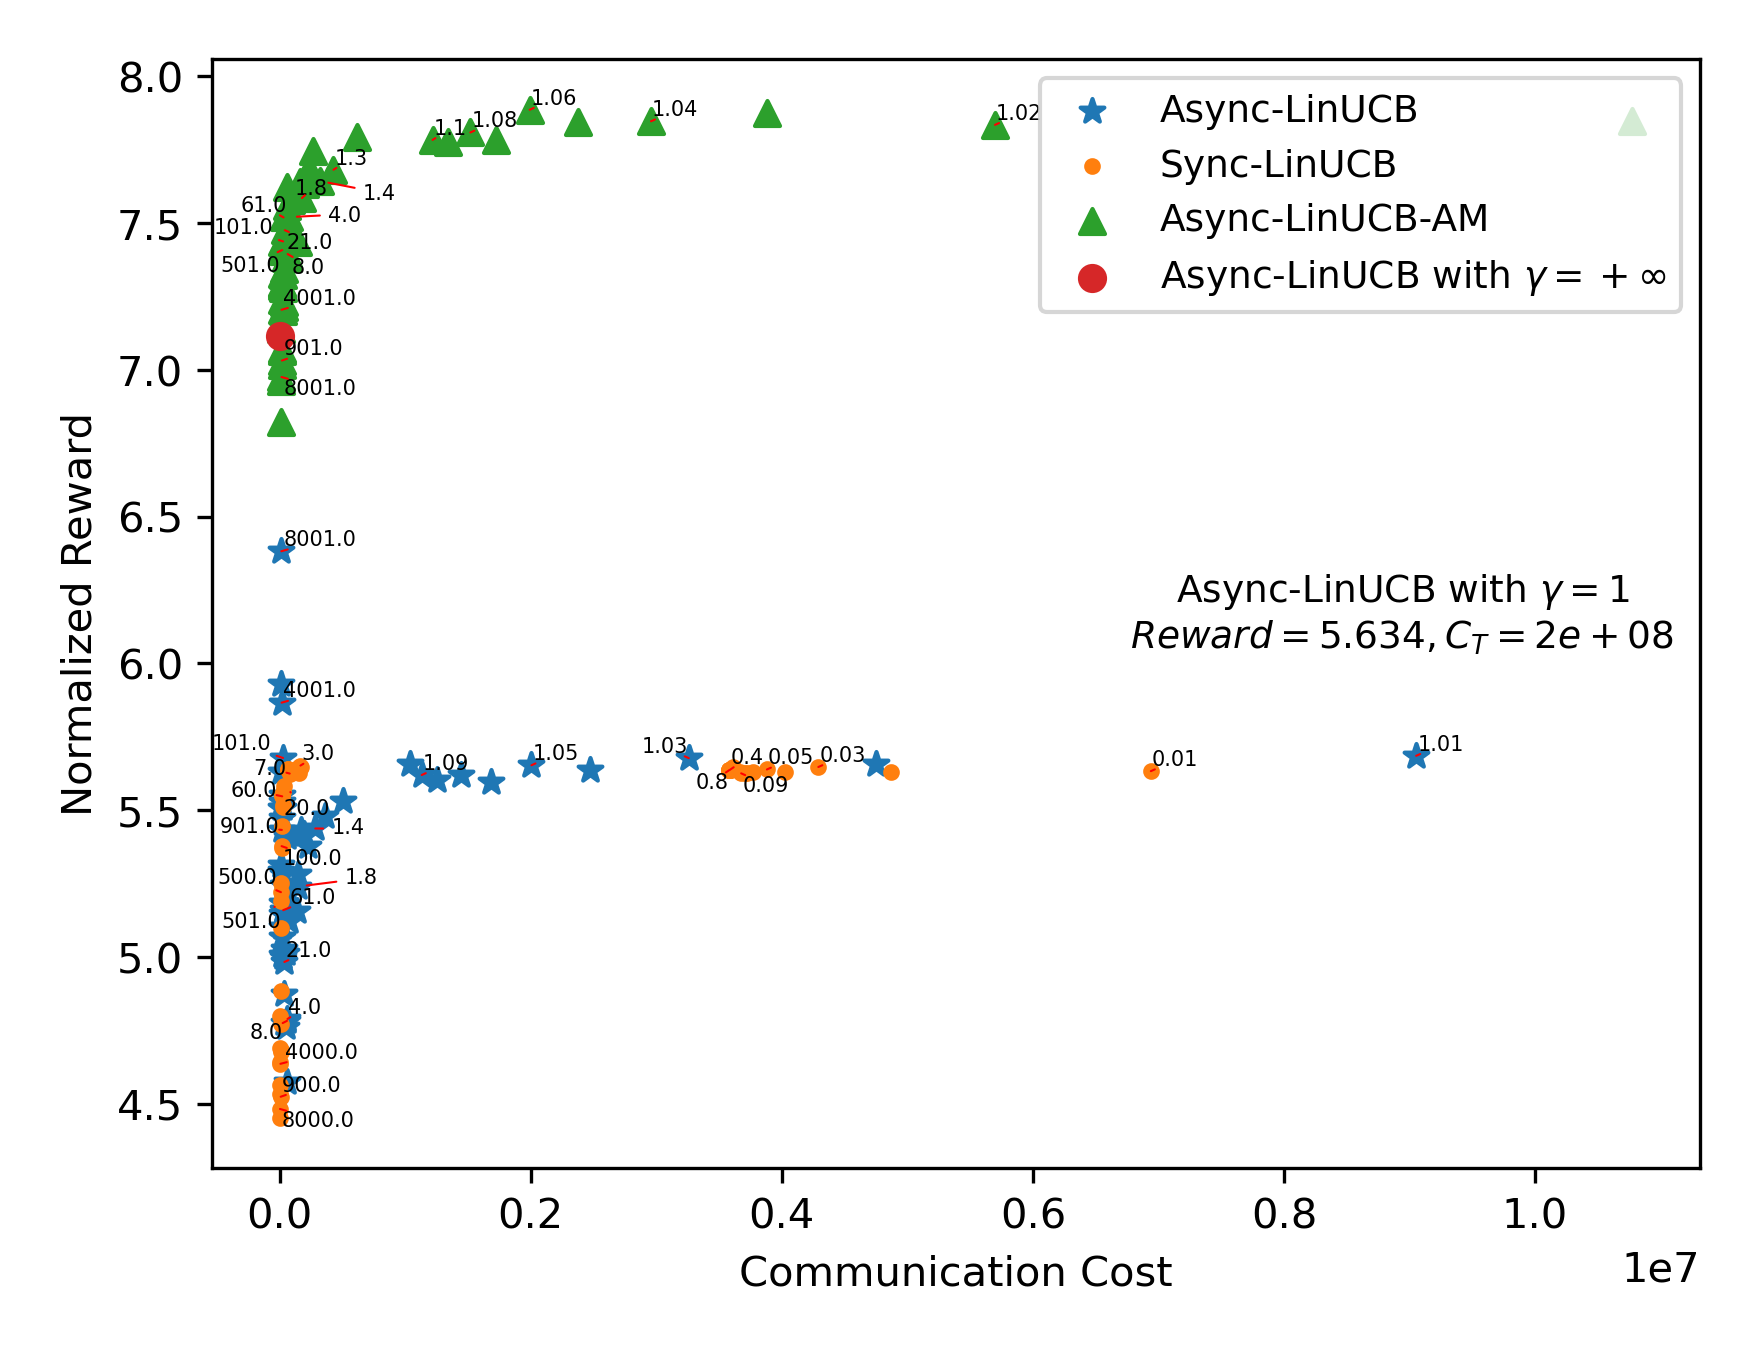
\includegraphics[width=0.48\textwidth]{imgs/regretVScommCost_lastfm_noclutter.png}}
% \medskip
% \subfigure[Delicious ($N=1867$)]{\label{fig:e}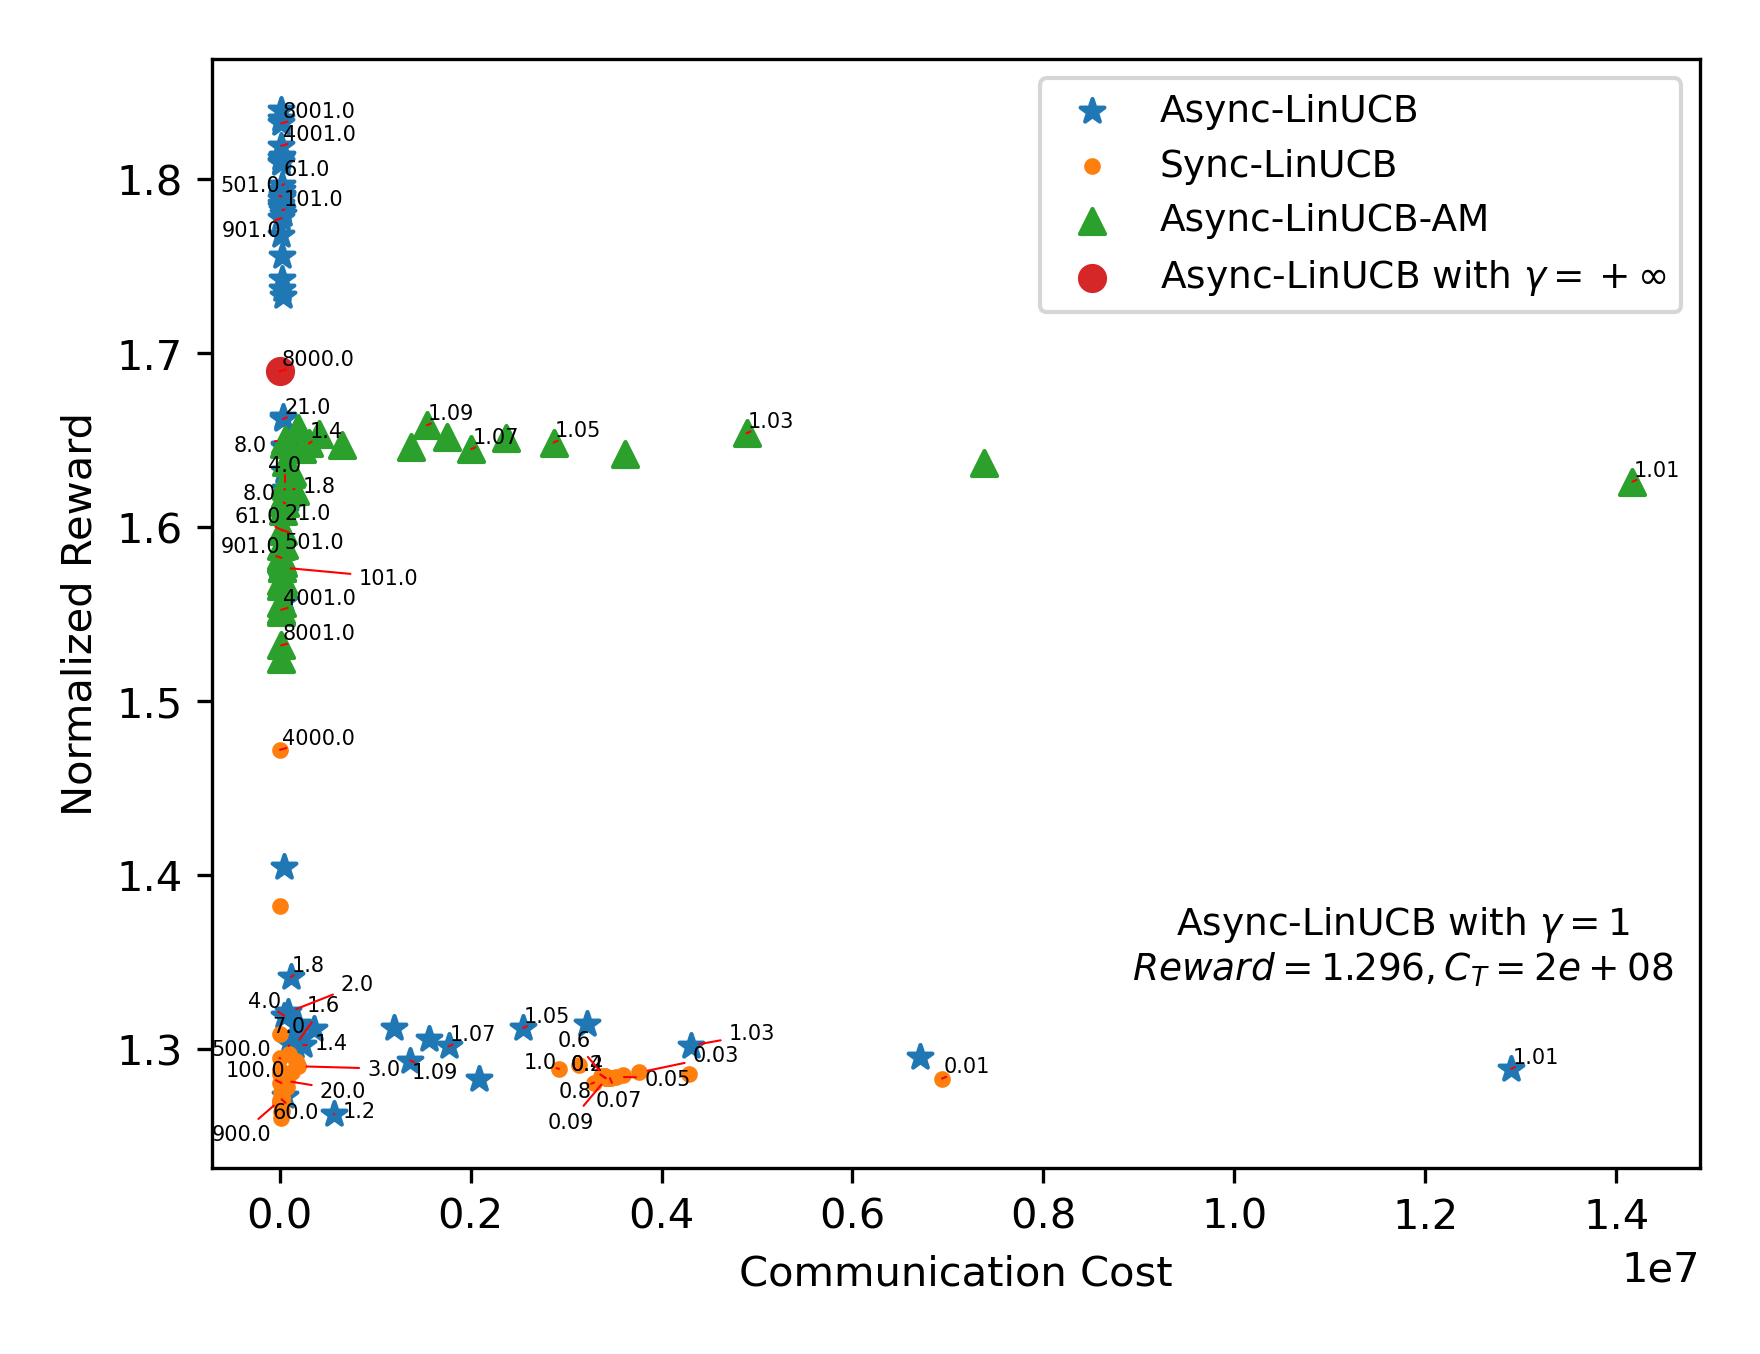
\includegraphics[width=0.48\textwidth]{imgs/regretVScommCost_delicious_noclutter.png}}
% \subfigure[MovieLens ($N=54$)]{\label{fig:f}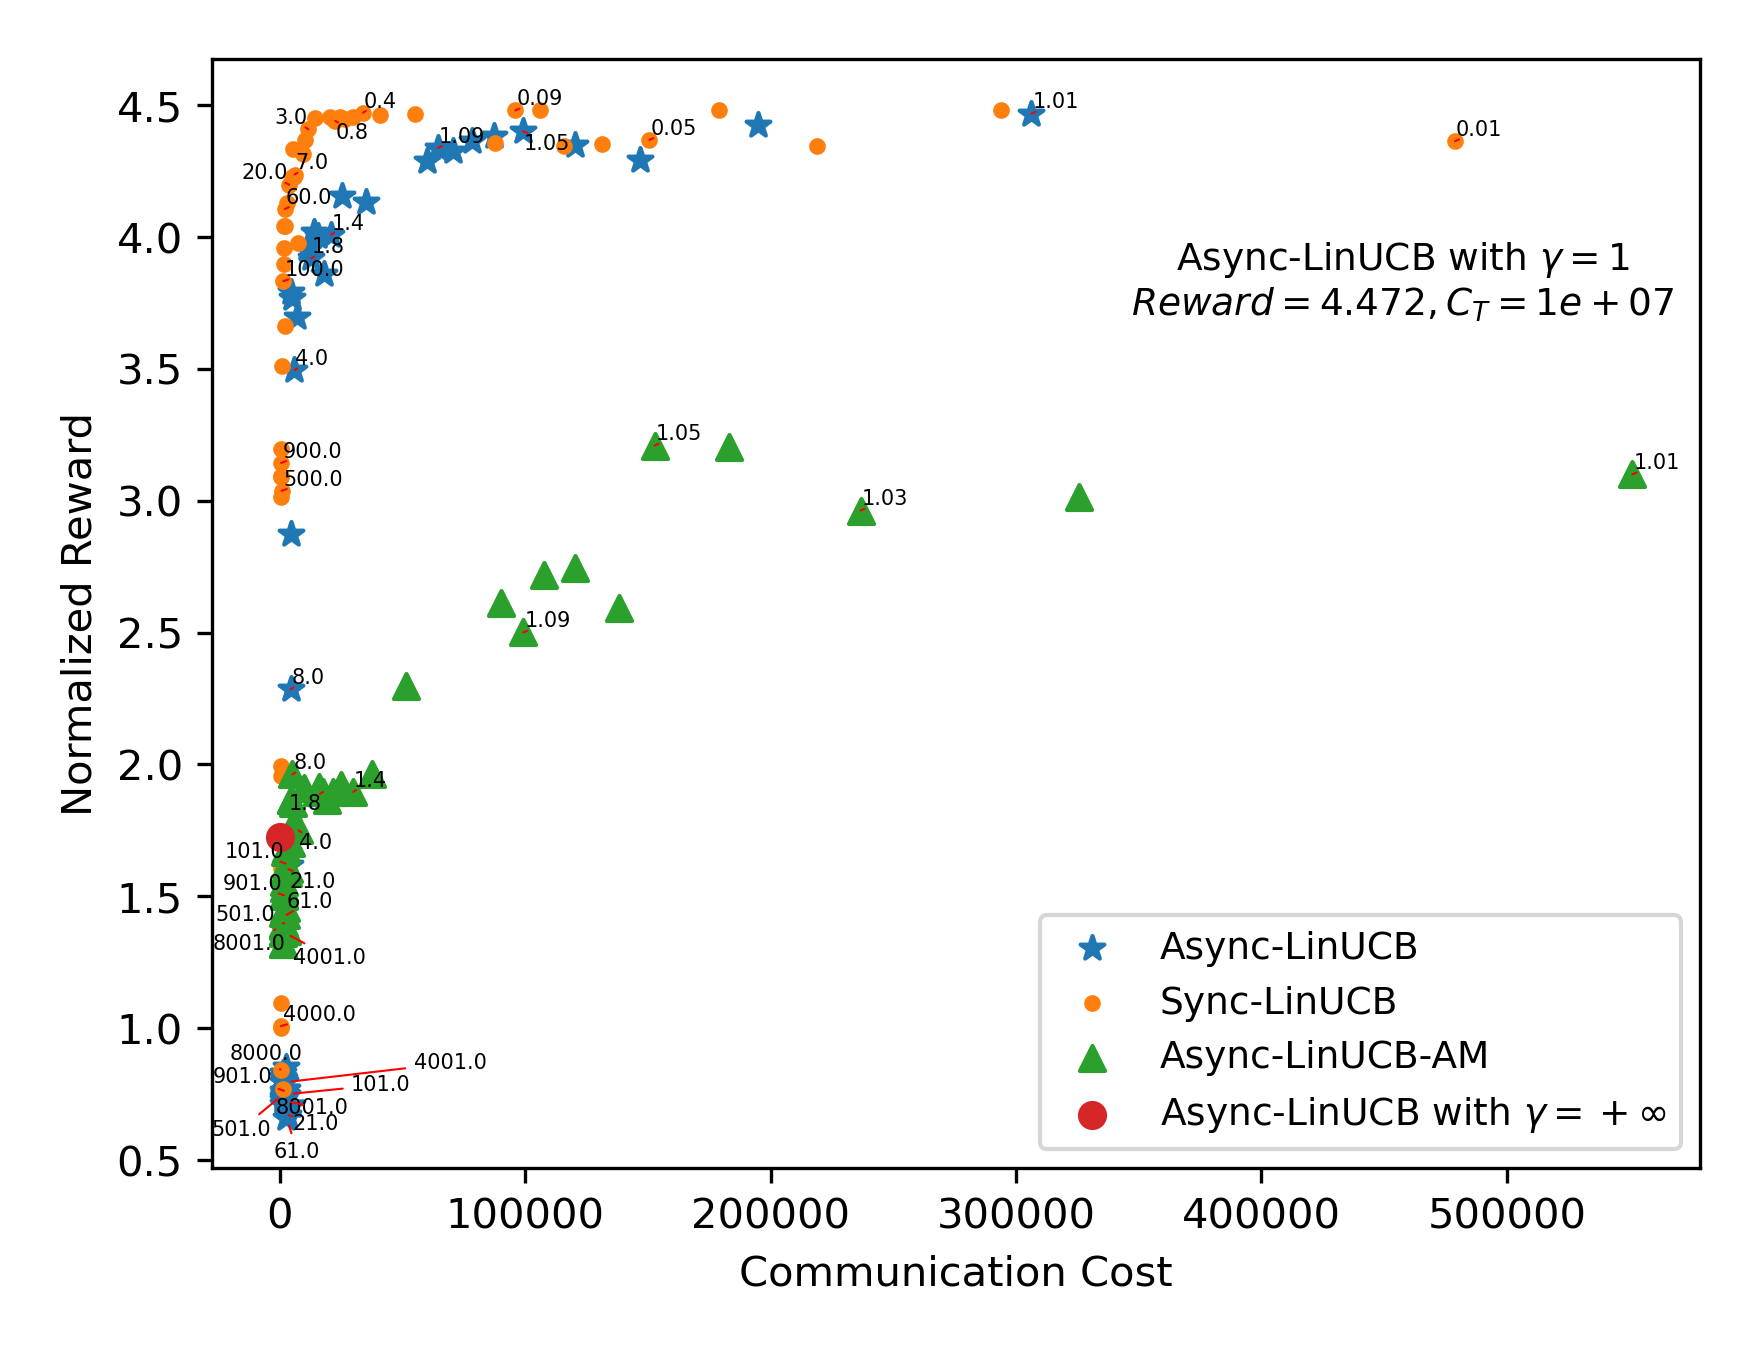
\includegraphics[width=0.48\textwidth]{imgs/regretVScommCost_movielens_noclutter.png}}
\vspace{-1mm}
\caption{Experiment results on synthetic dataset.}
\end{figure}

(1) Homogeneous clients (Figure \ref{fig:a}-\ref{fig:b}): 
From both Figure \ref{fig:a} and Figure \ref{fig:b}, we can see that as the threshold value increases, $C_{T}$ decreases and $R_{T}$ increases, and that the use of event-triggered communication significantly reduces $C_{T}$ while attaining low $R_{T}$, compared with synchronizing all the clients at each time step (\modelone{} with $\gamma=1$). In Figure \ref{fig:a}, \modelbaseline{} has lower $C_{T}$ than \modelone{} under the same $R_{T}$, and in Figure \ref{fig:b}, \modelone{} has lower $C_{T}$ than \modelbaseline{} under the same $R_{T}$, which conform with our theoretical results that \modelbaseline{} has inefficient communication under non-uniform client distribution.
% Among all the algorithms compared, \modelone{} with $\gamma=5$ and $\gamma=8$ and \modelbaseline{} with $D=\frac{T}{d \log{T}}$ strike a good balance between regret and communication cost. The other algorithms either incur a very high regret, i.e. \modelone{} with $\gamma=+\infty$ (as no communication can be triggered), or incur too much communication cost, i.e., \modelone{} with $\gamma=1$ and \modelbaseline{} with $D=\frac{T}{d N \log{T}}$ (as they always communicate). And almost in all results, both synthetic and real-world datasets, always communicating (i.e., \modelone{} with $\gamma=1$) costs significant overhead in communication, while it does not necessarily lead to an obvious advantage in regret. This suggests the necessity and benefit of our event-triggered communication control. In addition, the results for \modelbaseline{} with $D=\frac{T}{d N \log{T}}$ and $D=\frac{T}{d \log{T}}$ conform with our theoretical analysis in Remark \ref{rmk:regret_comm}, e.g., it incurs higher regret when matching the communication cost with \modelone{} or higher communication cost when matching the regret with \modelone{}. 
% \modelone{} with $\gamma=1$ and \modelbaseline{} with $D=\frac{T}{d N \log{T}}$ attain the lowest regret, but also incur much higher communication costs compared with other algorithms.

(2) Heterogeneous clients (Figure \ref{fig:c}): By increasing the portion of global components $\theta^{g}$ in the bandit parameter, we can observe a clear trend in both regret and communication cost, i.e., the regret keeps decreasing while the communication cost keeps increasing. This validates our theoretical analysis about $R_{T}$ and $C_{T}$ in Section \ref{subsec:async_LinUCB_AM}. With $d_{g}$ increases and $d_{l}$ decreases, the first term in the upper bound of $R_{T}$ dominates (which grows slower w.r.t. $N$ compared with the second term), leading to the decreased regret, but the communication cost would increase since $C_{T}=O(d_{g} N \log{T})$.

\subsection{Experiments on Real-world Dataset}
% From the experiments on synthetic dataset, we have validated our upper bounds on the regret and communication cost of \modelone{} and \modeltwo{}. 
%However, we should note that our theoretical results are based on a slightly stronger assumption on the context vectors (see Assumption \ref{assump:context_diversity}), compared with \modelbaseline{}. 
%Therefore, we want to validate whether such an assumption is reasonable in practice, i.e., whether our algorithms can still work properly on the real-world datasets that contain TF-IDF feature vectors extracted from the tags and metadata of the items. 
We continue investigating the effectiveness of our proposed solution on real-world datasets. Note that these real-world datasets do not necessarily satisfy the assumption that all the clients are homogeneous, in other words not all the users have the same preference, we pay special attention to \modeltwo{} in the comparison, by setting $x_{g} \equiv x_{i}, \forall i \in [N]$, as mentioned in Section \ref{subsec:problem_formulation}. This allows the clients to learn a global model collaboratively, and in the meantime each learns a personalized model independently. Intuitively, this should make \modeltwo{} more robust to different settings, i.e., the clients are either homogeneous or heterogeneous.
\subsubsection{Real-world dataset.}
We compared \modelone{}, \modeltwo{} and \modelbaseline{} on three public recommendation datasets: LastFM, Delicious and MovieLens \citep{Cantador:RecSys2011,harper2015movielens}, with various threshold values (logarithmically spaced between $10^{-2}$ and $10^{3}$). 
The LastFM dataset contains $N=1892$ users, 17632 items (artists), and $T=96733$ interactions. We consider the ``\textit{listened artists}'' in each user as positive feedback. The Delicious dataset contains $N=1861$ users, 69226 items (URLs), and $T=104799$ interactions. We treat the bookmarked URLs in each user as positive feedback. 
The MovieLens dataset used in the experiment is extracted from the MovieLens 20M dataset by keeping users with over $3000$ observations, which results in a dataset with $N=54$ users, 26567 items (movies), and $T=214729$ interactions. We consider all items with non-zero ratings as positive feedback. The datasets were preprocessed following the procedure in \cite{cesa2013gang} to fit the linear bandit setting (with TF-IDF feature $d=25$ and arm set $K=25$).
% When applying \modeltwo{}, we assumed $x_{g} \equiv x_{i}, \forall i \in [N]$, as mentioned in Section \ref{subsec:problem_formulation}.
% We compare \modelone{} (with $\gamma \in \{1,5,+\infty\}$), \modeltwo{} (with $\gamma=5$) and \modelbaseline{} (with $D \in \{\frac{T}{d N \log{T}}, \frac{T}{d \log{T}}\}$) on three public recommendation datasets: LastFM, Delicious and MovieLens \cite{Cantador:RecSys2011,harper2015movielens}, with normalized reward (by a random strategy) and communication cost reported in Figure \ref{fig:exp_result}(c)-(e). When applying \modeltwo{}, we assume $x_{g} \equiv x_{i}, \forall i \in [N]$, as mentioned in Section \ref{subsec:problem_formulation}. The datasets are preprocessed following the procedure in \cite{cesa2013gang} to fit the linear bandit setting (with TF-IDF feature $d=25$ and arm set $K=25$).

% \subsubsection{Real-world dataset.}
% The three real-world datasets used in our experiment, i.e., LastFM, Delicious and MovieLens, are public recommendation datasets. Specifically, the LastFM dataset was extracted from the music streaming service Last.fm, and the Delicious dataset was extracted from the social bookmark sharing service Delicious. They were made availalbe by the HetRec 2011 workshop. The LastFM dataset contains $N=1892$ users, 17632 items (artists), and $T=96733$ interactions. We consider the ``\textit{listened artists}'' in each user as positive feedback. The Delicious dataset contains $N=1861$ users, 69226 items (URLs), and $T=104799$ interactions. We treat the bookmarked URLs in each user as positive feedback. 
% The MovieLens dataset used in the experiment is extracted from the MovieLens 20M dataset by keeping users with over $3000$ observations, which results in a dataset with $N=54$ users, 26567 items (movies), and $T=214729$ interactions.
% % that contains 20 million ratings with 27,000 movies and 138,000 users.
% % the MovieLens 20M dataset by keeping users with denser observations, which results in 54 users and 26567 items (movies).
% We consider all items with non-zero ratings as positive feedback in this dataset.
% On the LastFM and Delicious datasets, we extracted TF-IDF feature vectors using tags associated with each item; and on the MovieLens dataset, we also used information from items' metadata, such as movie titles, genres, etc., in addition to the tags, to construct the context vector. We then applied PCA to the resulting TF-IDF feature vectors, and retained the first 25 principle components as the context vectors, i.e., $d=25$. Then we normalized all features to have a zero mean and unit variance in each dimension. To generate the interaction sequence for each user, at each time step when a particular user $i_{t}$ is served, the candidate arm pool for user $i_{t}$ is generated by keeping the item with positive feedback at this time step and sampling another 24 unrated/non-interacted items from this user, i.e., $K=25$.

\subsubsection{Experiment results.}
% \textbf{Results on real-world datasets}:
%First, from the results on all three datasets (Figure \ref{fig:d}-\ref{fig:f}), the performance of \modelone{} is as good as that of \modelbaseline{}, which indicates Assumption \ref{assump:context_diversity} is still reasonable with the TF-IDF feature vectors. Especially in the results on MovieLens dataset (Figure \ref{fig:f}), whose data conforms with our homogeneous clients assumption as we will see below, we can see the dots corresponding to \modelone{} and \modelbaseline{} have very similar patterns as that in the ideal simulation environment (Figure \ref{fig:a}).

Experiment results on the three real-world datasets are shown in Figure \ref{fig:d}-\ref{fig:f}. 
In the scatter plots, each dot denotes the cumulative communication cost (x-axis) and normalized reward by a random strategy (y-axis) that an algorithm (\modelone{}, \modeltwo{}, or \modelbaseline{}) with certain threshold value (labeled next to the dot) has obtained at iteration $T$.
To understand the results of these algorithms on the three real-world datasets, we can first look at how well the two extreme cases, \modelone{} with $\gamma=1$ (as the communication cost of this algorithm is outside of the figure, its result is illustrated as text label) and \modelone{} with $\gamma=+\infty$ perform. 

\begin{figure}
\centering     %%% not \center
% \subfigure[Homogeneous (uniform)]{\label{fig:a}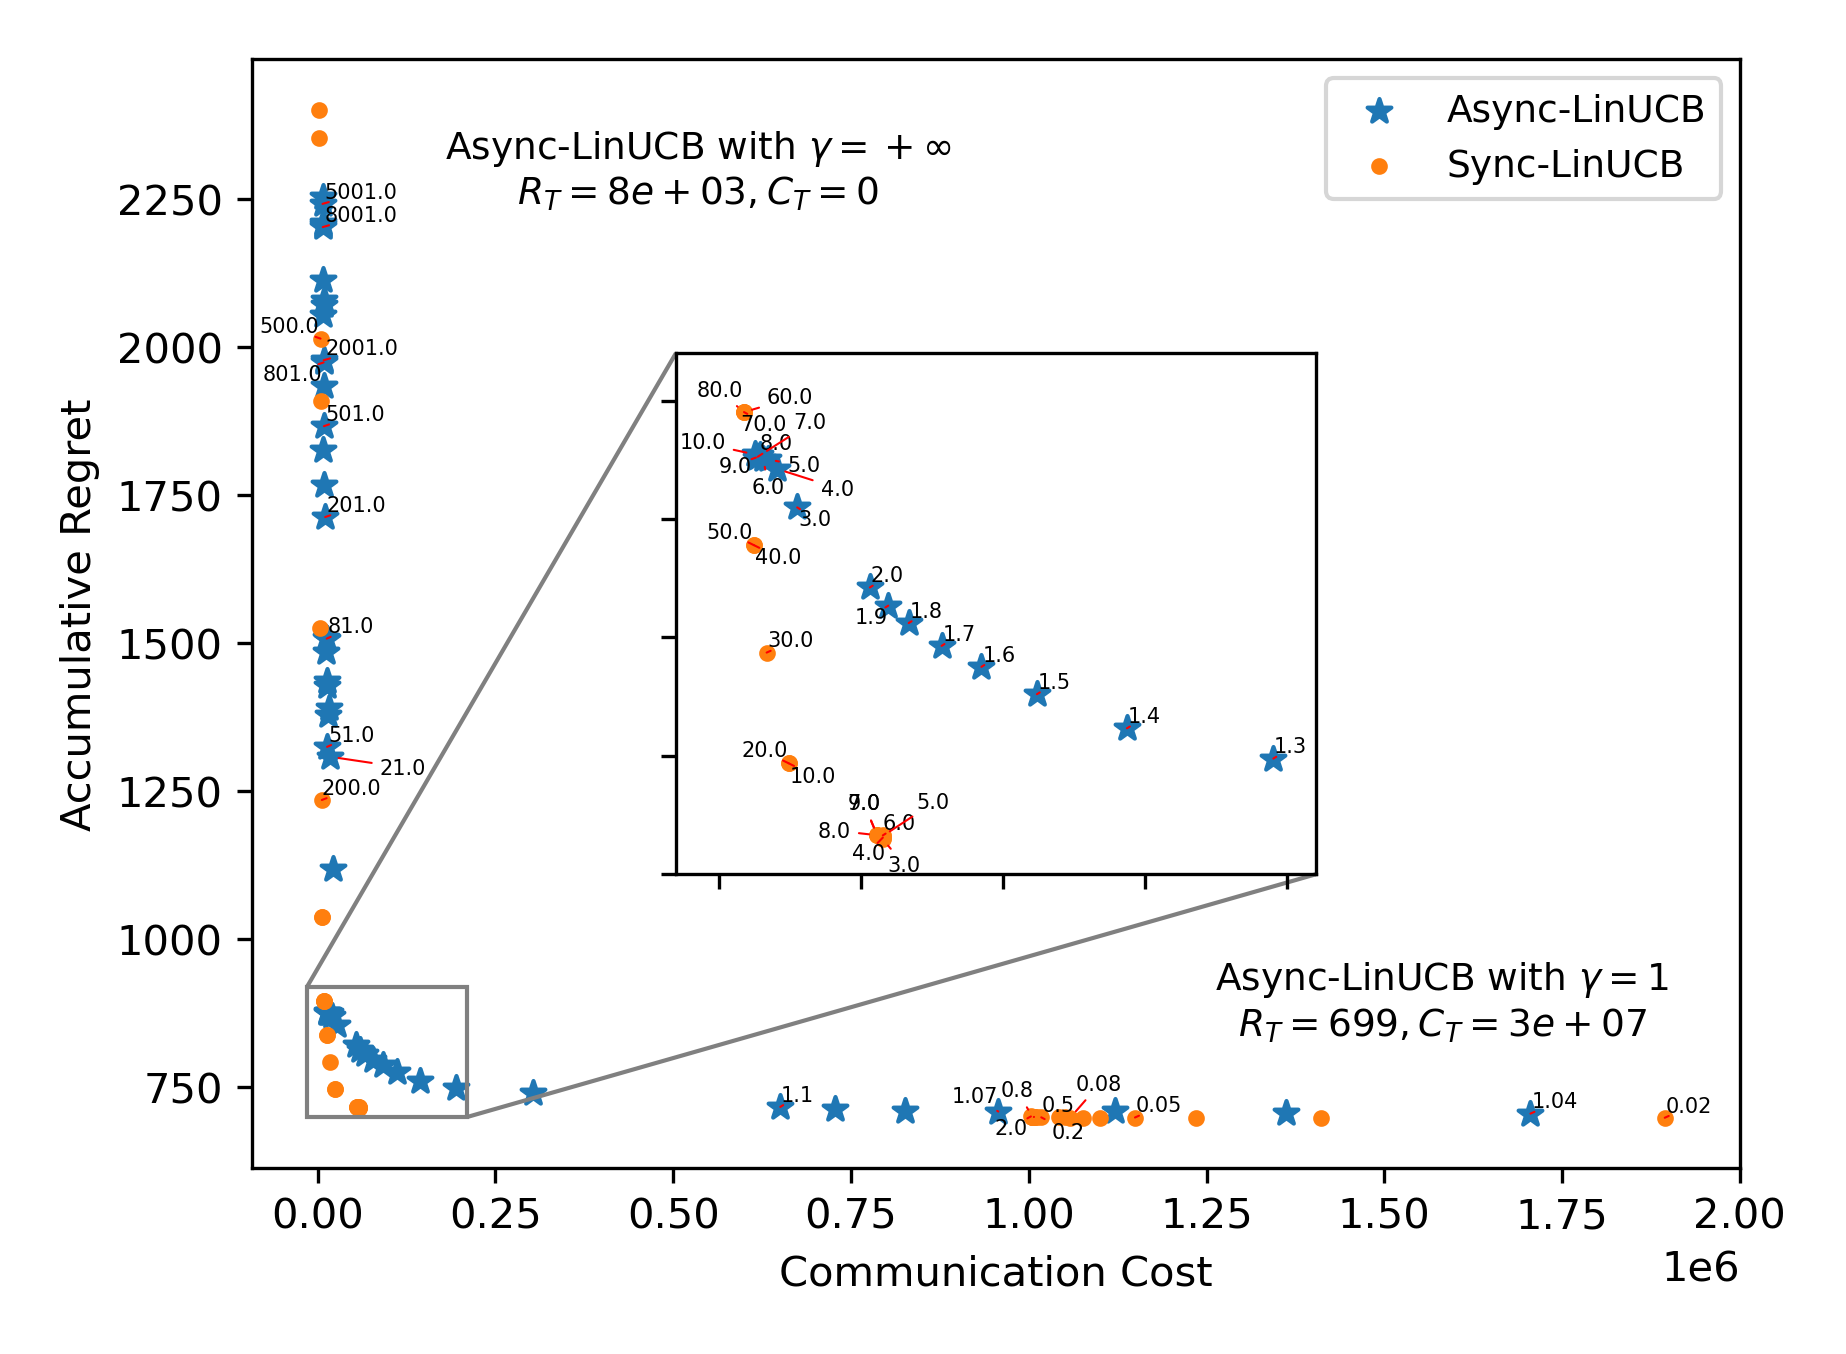
\includegraphics[width=0.48\textwidth]{imgs/regretVScommCost_uniform_noclutter.png}}
% \subfigure[Homogeneous (non-uniform)]{\label{fig:b}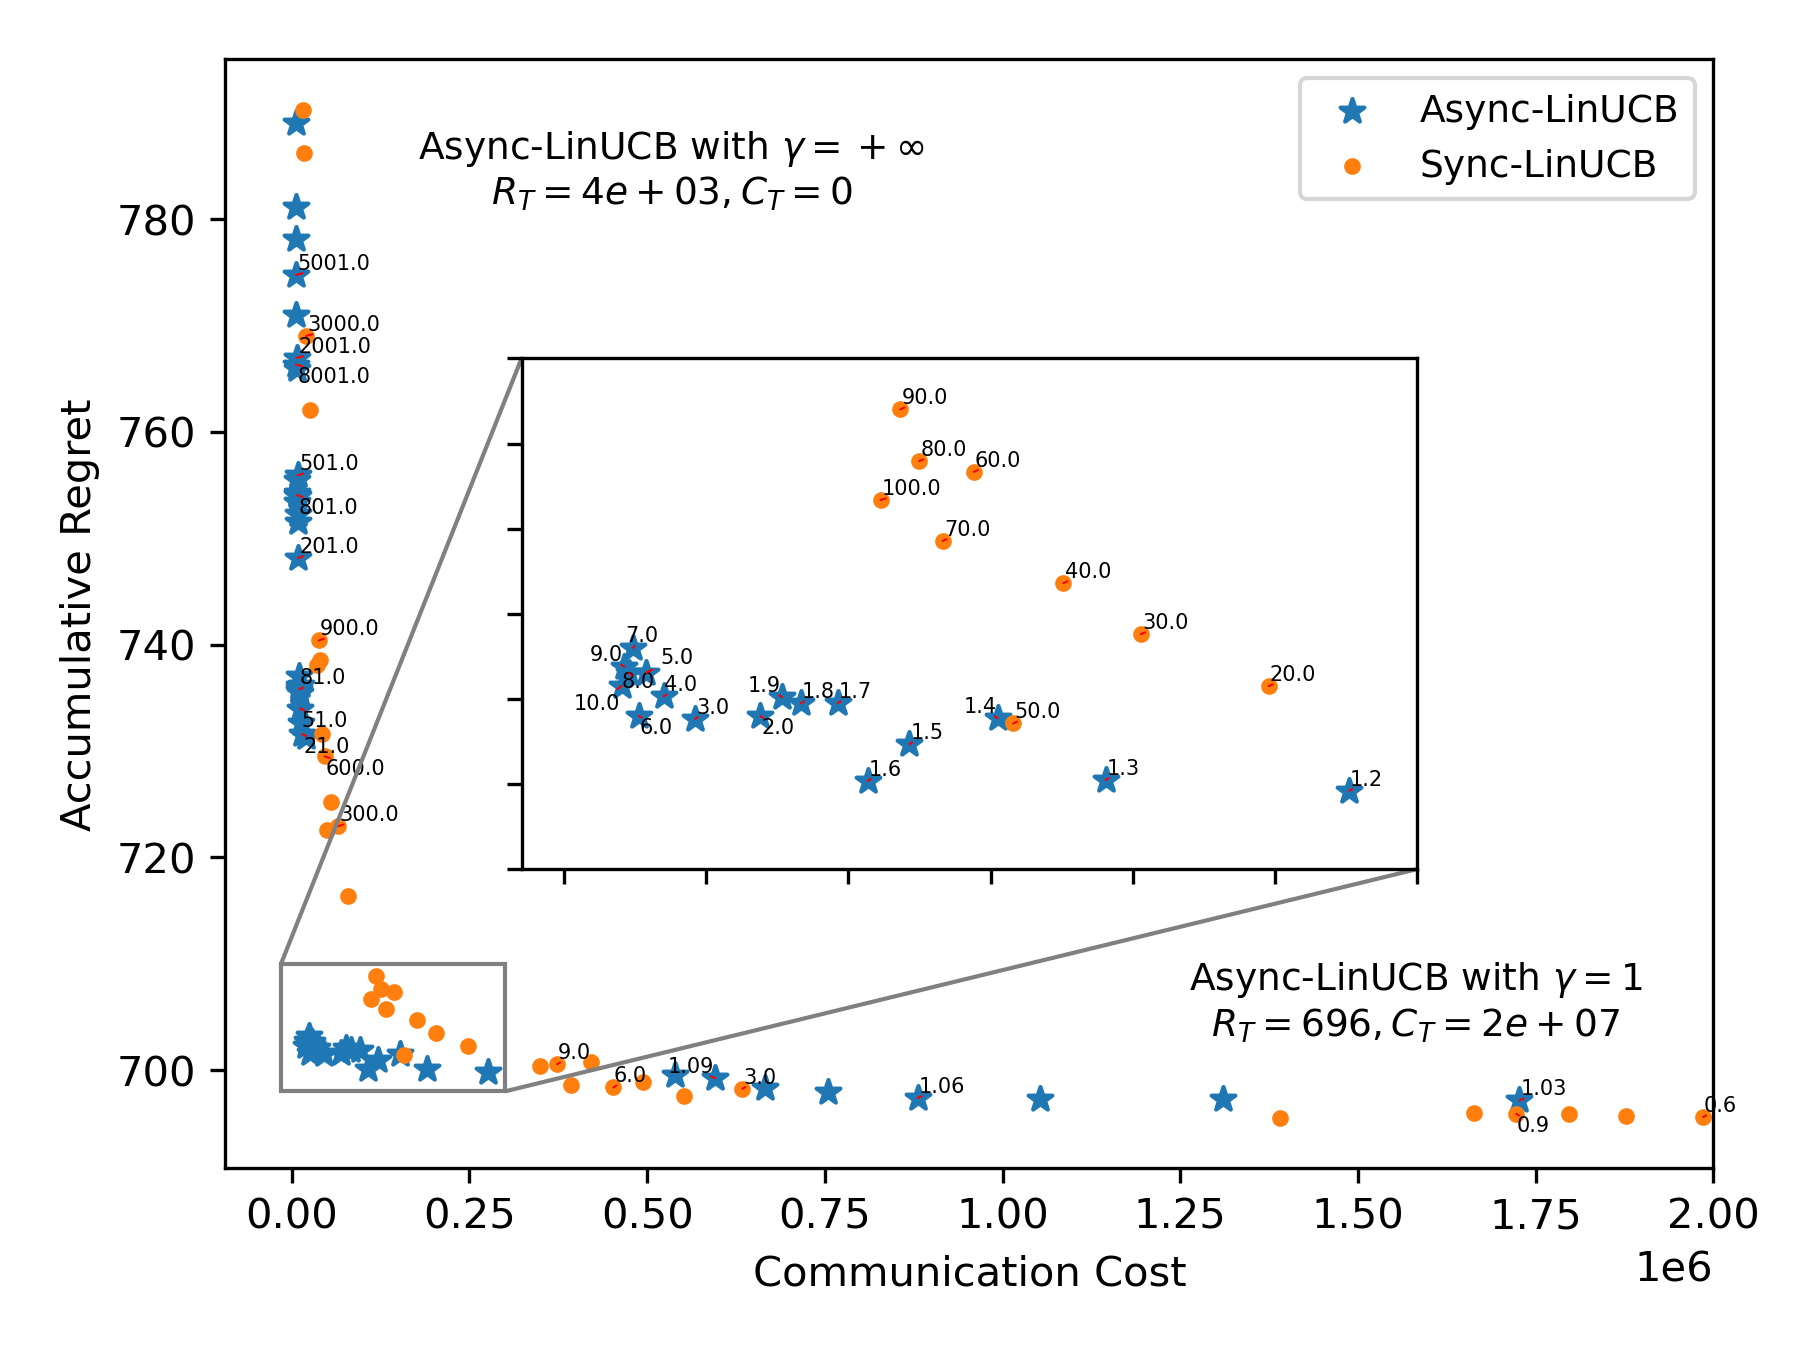
\includegraphics[width=0.48\textwidth]{imgs/regretVScommCost_nonuniform_noclutter.png}}
% % \vspace{-1mm}
% \medskip
% \subfigure[Heterogeneous clients]{\label{fig:c}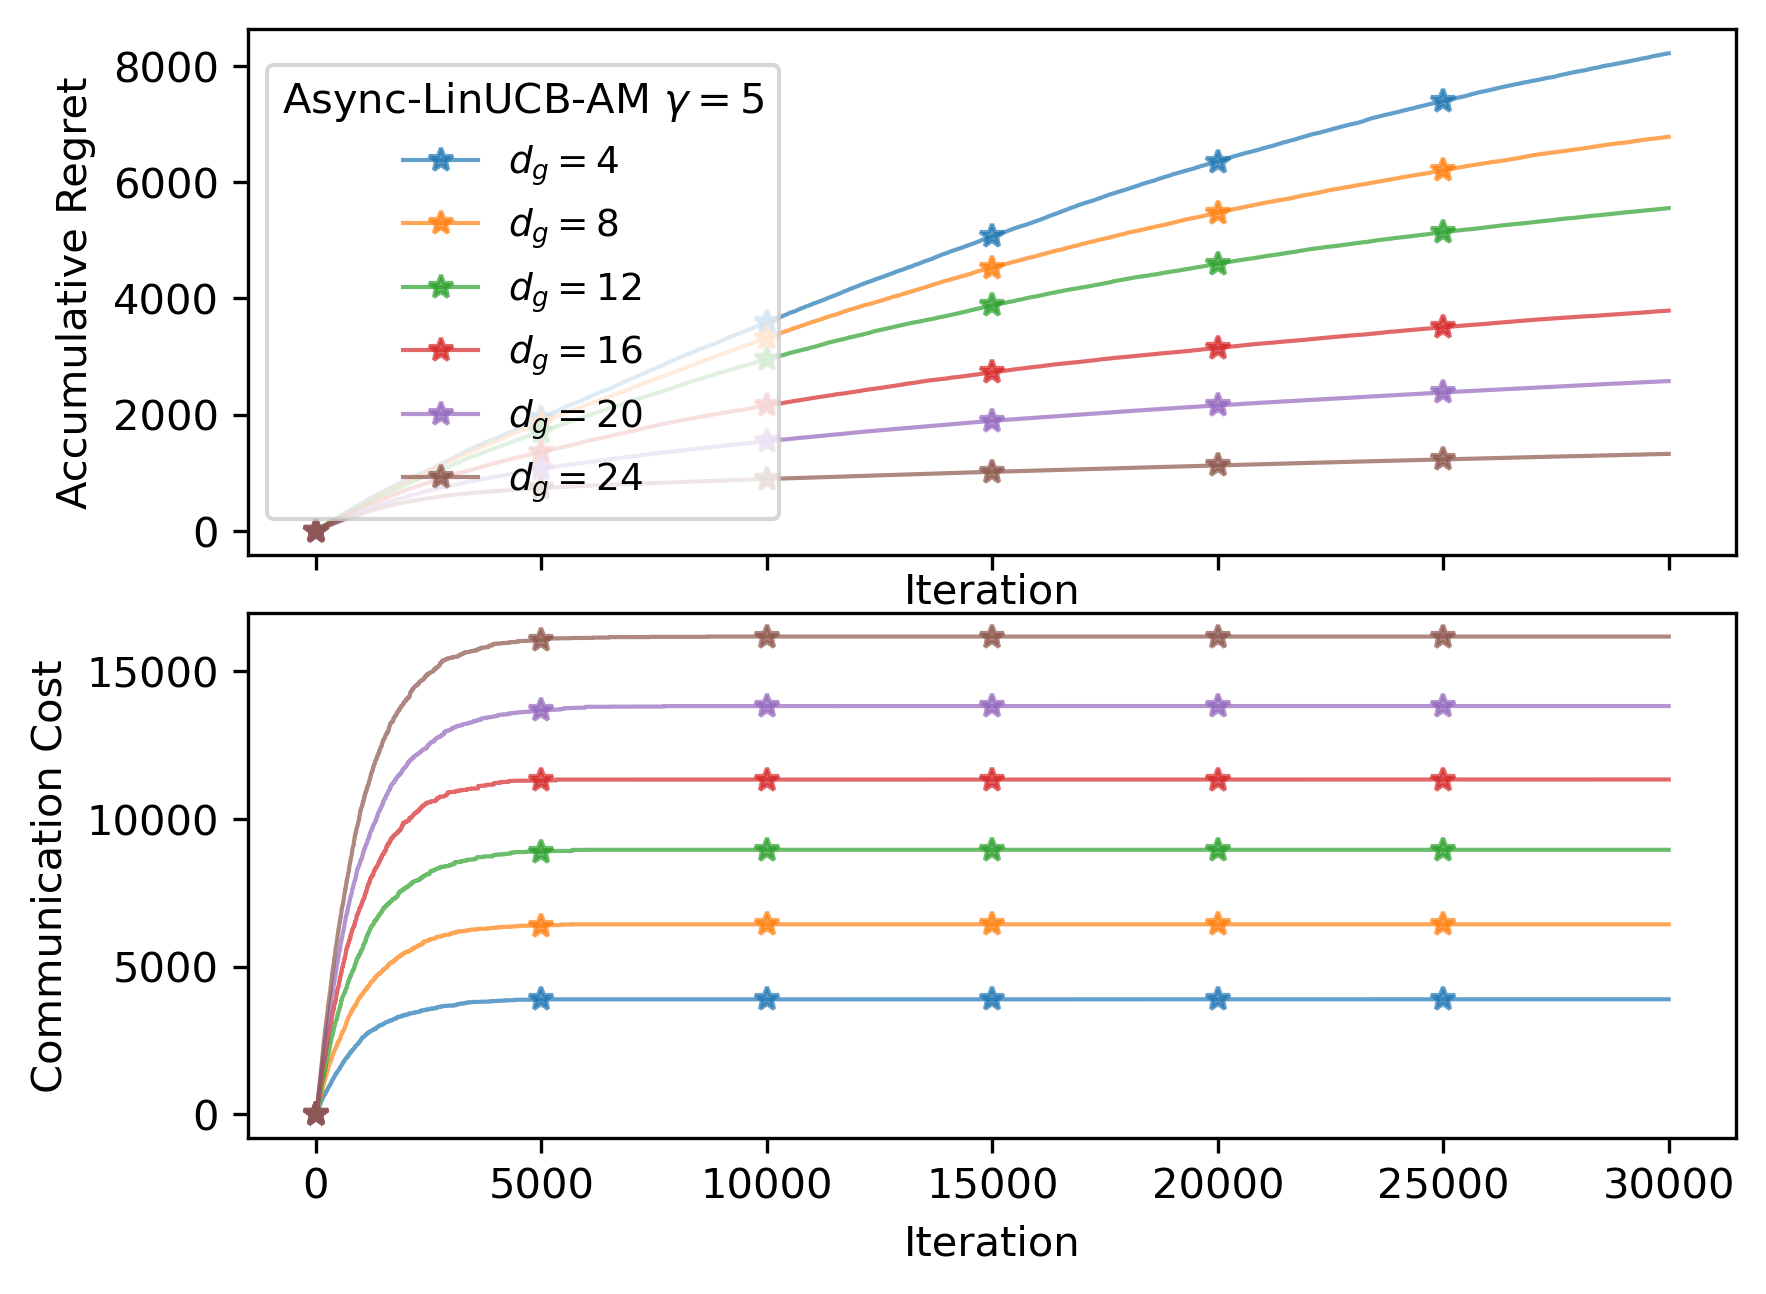
\includegraphics[width=0.48\textwidth]{imgs/sim_hetero_30000.png}}
\vspace{-2mm}
\subfigure[LastFM ($N=1892$)]{\label{fig:d}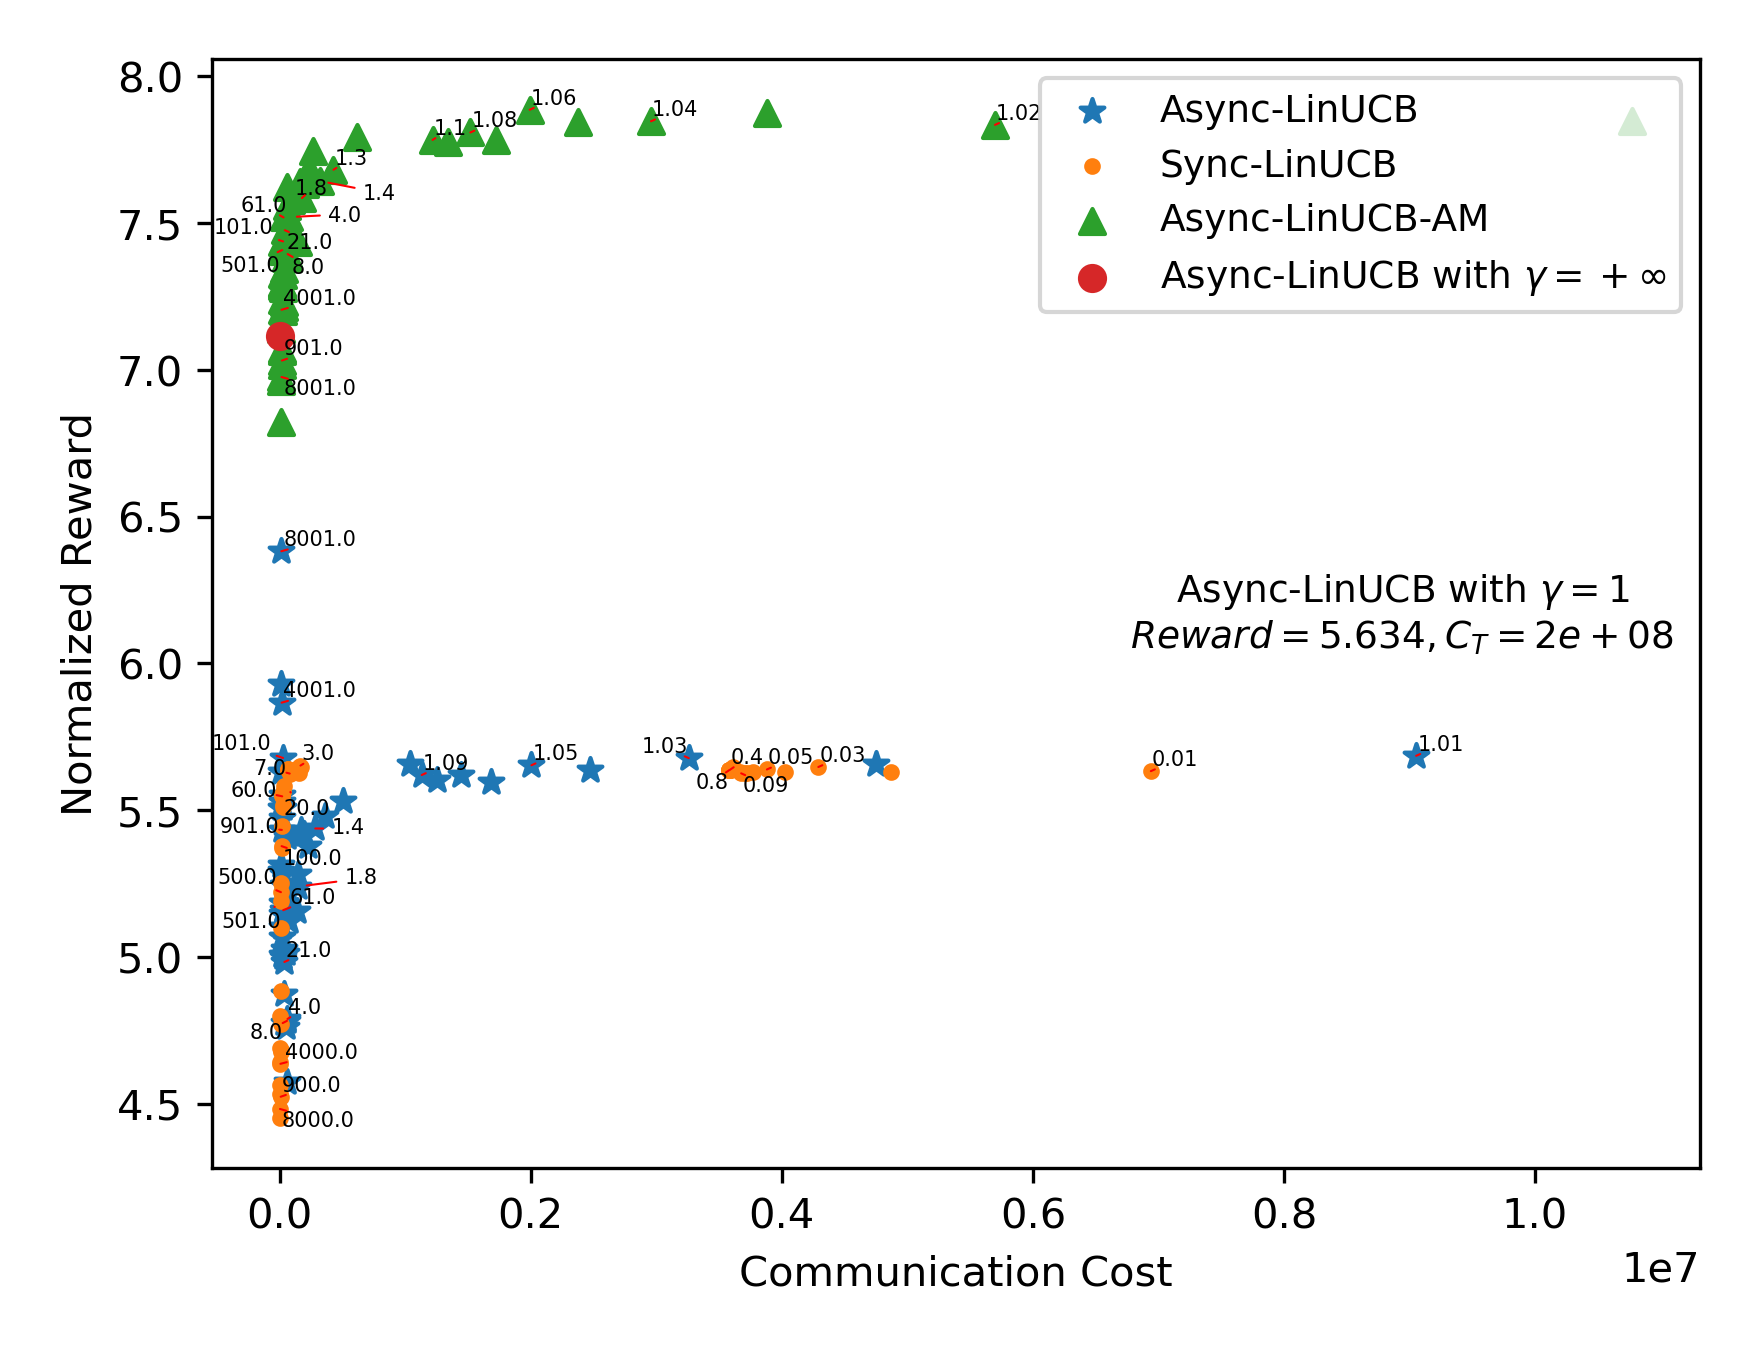
\includegraphics[width=0.55\textwidth]{imgs/regretVScommCost_lastfm_noclutter.png}}
\vspace{-2mm}
\subfigure[Delicious ($N=1867$)]{\label{fig:e}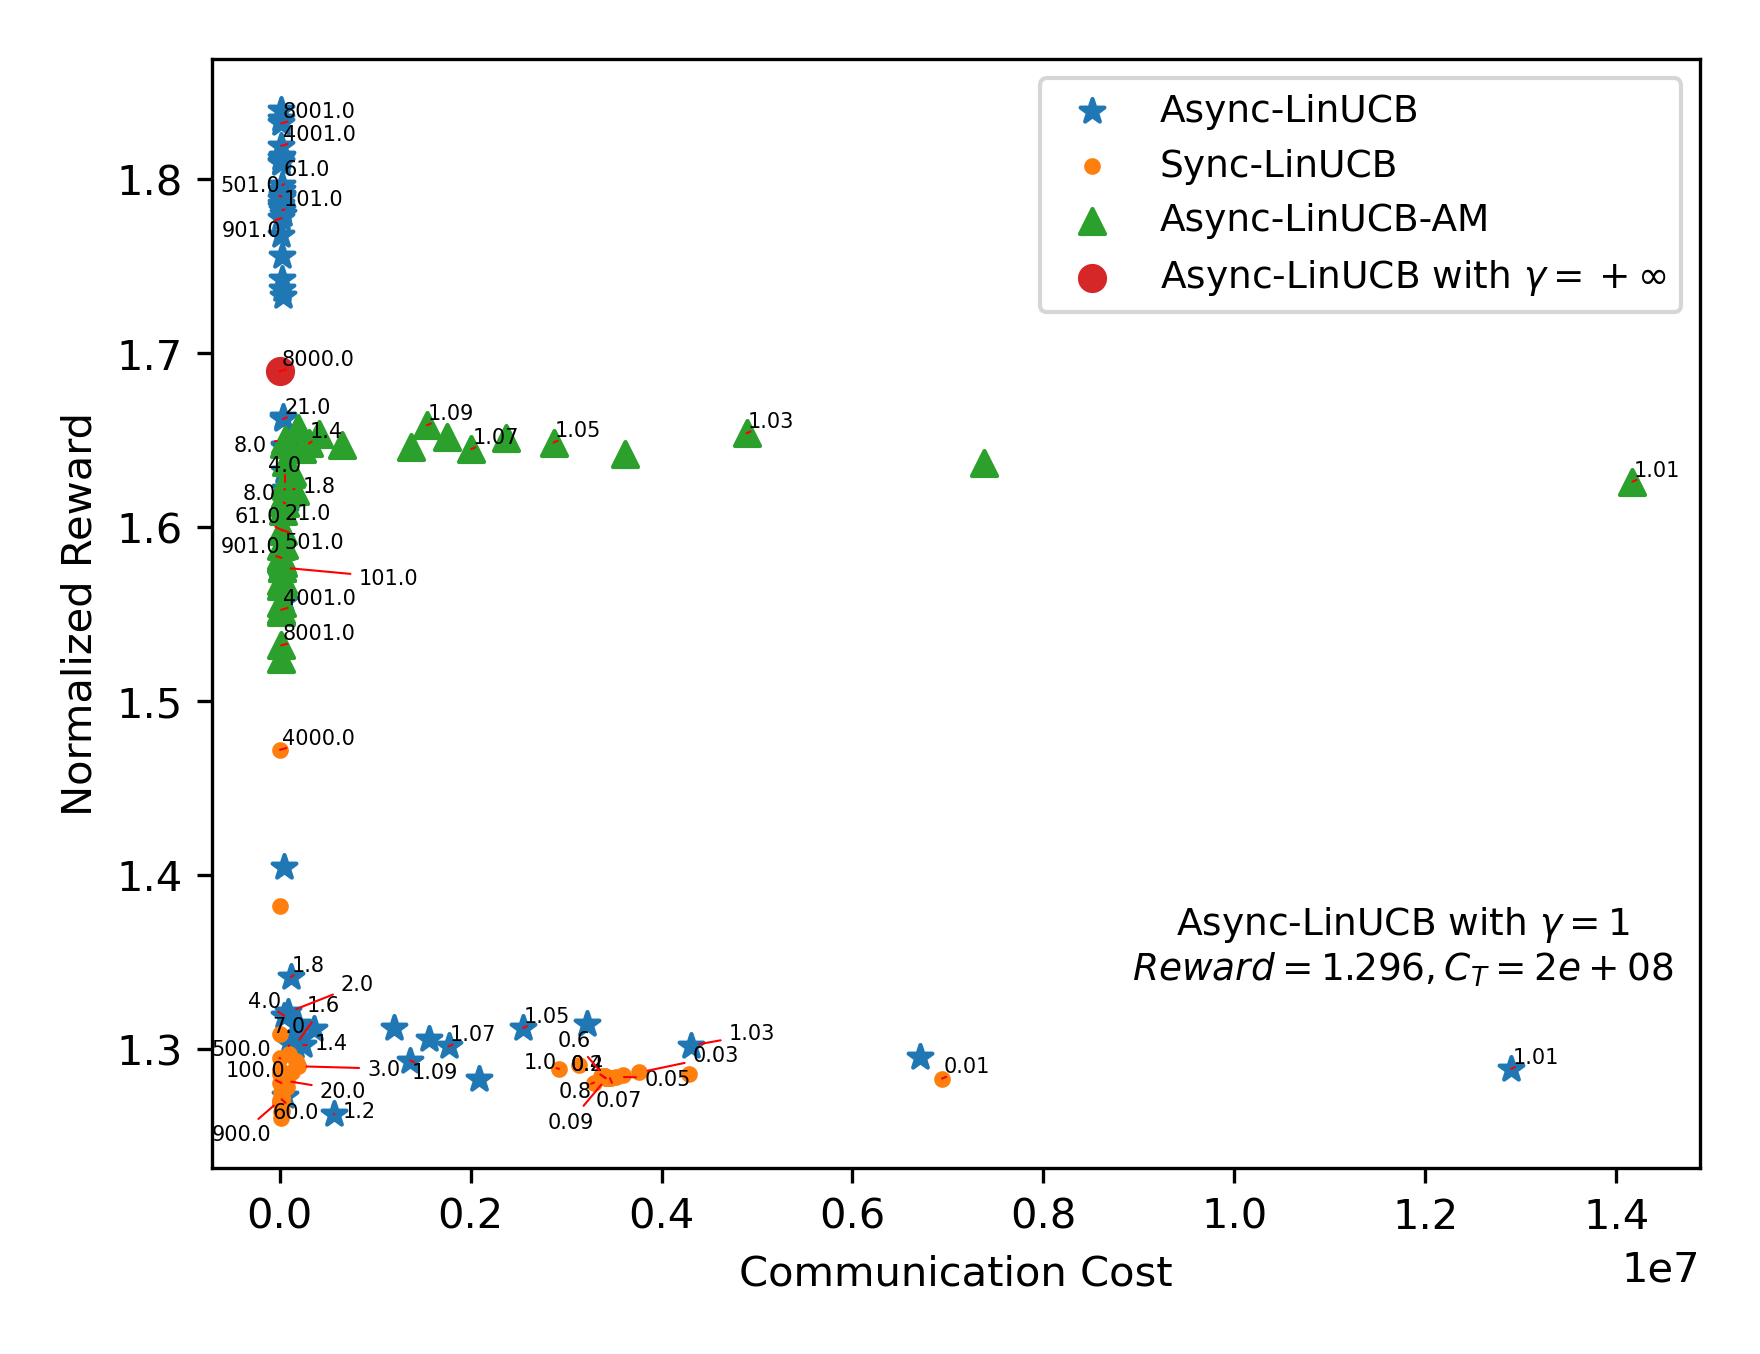
\includegraphics[width=0.55\textwidth]{imgs/regretVScommCost_delicious_noclutter.png}}
\vspace{-2mm}
\subfigure[MovieLens ($N=54$)]{\label{fig:f}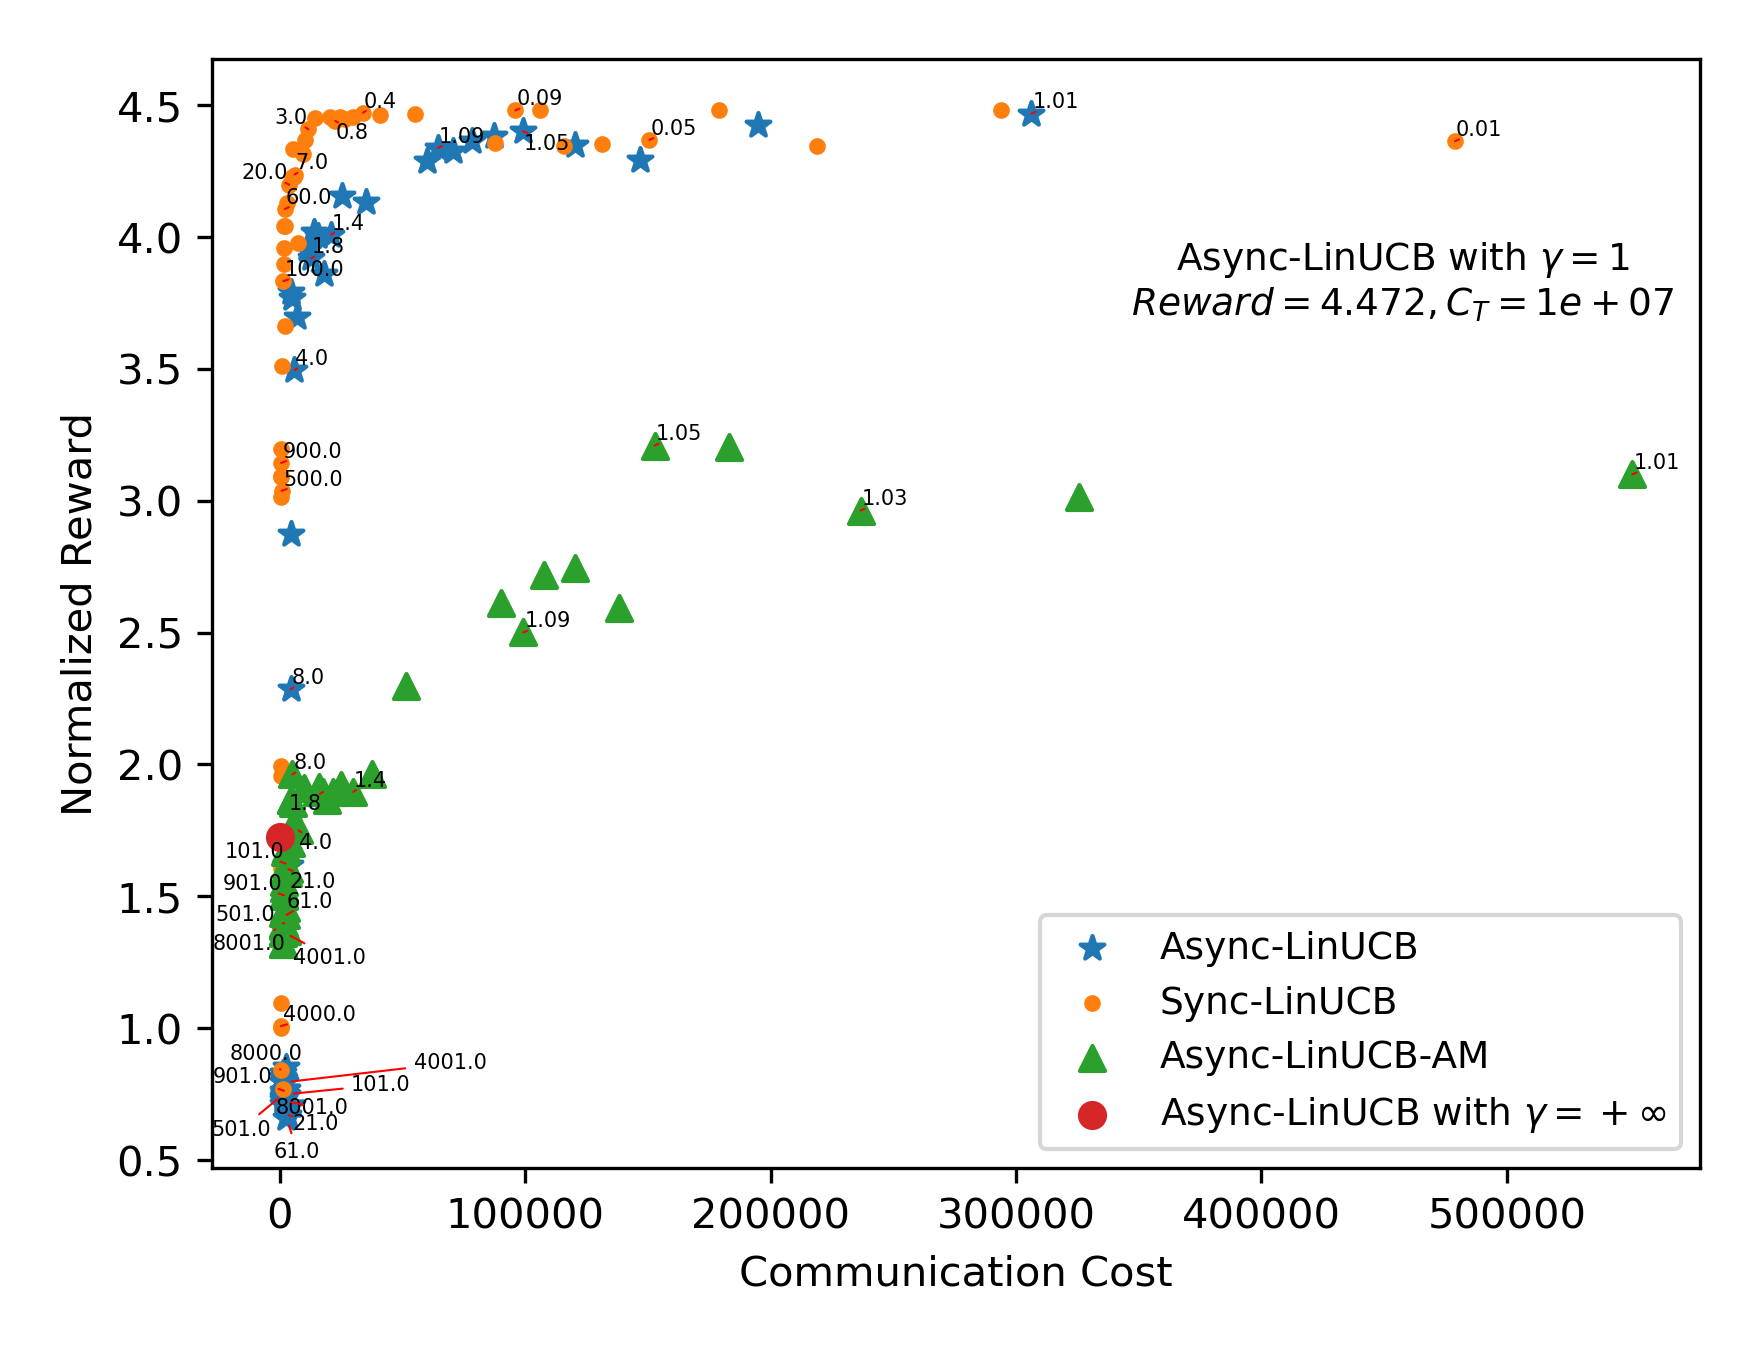
\includegraphics[width=0.55\textwidth]{imgs/regretVScommCost_movielens_noclutter.png}}
% \vspace{-1mm}
\caption{Experiment results on real-world recommendation datasets.}
\end{figure}

(1) LastFM \& Delicious (Figure \ref{fig:d}-\ref{fig:e}): 
On both LastFM and Delicious datasets, \modelone{} with $\gamma=+\infty$ (illustrated as the red dot) attains very high reward, which suggests users in these two datasets have very diverse preferences, such that aggregating their data has a negative impact on the performance. 
Since the homogeneous clients assumption does not hold in this case, both \modelone{} and \modelbaseline{} perform as badly as the extreme case of \modelone{} with $\gamma=1$, which is especially true when the clients frequently communicate with each other, i.e., with lower threshold values.
% , and the more the clients communicate with each other, the lower rewards they will obtain, due to the mistakenly aggregated heterogeneous data. 
In comparison, \modeltwo{} attains relatively good performance even when the clients frequently communicate with each other, as it allows personalized models to be learned on each client. Note that on Delicious dataset, in the low communication/high threshold region (top left corner of Figure \ref{fig:e}), the reward of \modelone{} actually increases as communication increases. Our hypothesis is that, with high threshold, only the most active users contribute to global data sharing, and when the other less active clients download these data, the benefit from reduced variance outweighs the harm caused by the increased bias (due to user heterogeneity). However, with the threshold further reduced, many more clients are able to contribute to global data sharing, such that the global data would become so heterogeneous that it starts to hurt the overall performance. Additional experiment and visualization are given in appendix (Section \ref{sec:additional_exp}) to validate this hypothesis.

(2) MovieLens (Figure \ref{fig:f}): 
Note that on this dataset, \modelone{} with $\gamma=1$ attains very high reward, which indicates that the users share similar preferences, so that data aggregation over different users becomes vital for good performance. 
In this case, learning a personalized model on each client becomes unnecessary and slows down the convergence of model estimation, which leads to the lower accumulative reward of \modeltwo{} compared with the other two algorithms.
% And as \modeltwo{} requires each client to learn a personalized model, which becomes unnecessary in this case, 
% it slows down convergence of the model estimation and thus leads a lower reward compared with the other two algorithms.
However, we can see that \modeltwo{} can still benefit from collaborative model estimation, as it has a much higher accumulative reward than the extreme case of \modelone{} with $\gamma=+\infty$.